\documentclass[authoryearcitations]{UoYCSproject}

\usepackage[
    bindingoffset=13mm,
    includehead, includefoot,
    left=2cm, right=2cm, top=2cm, bottom=2cm
]{geometry}

\usepackage{tikz}
\usetikzlibrary{arrows,positioning}

\tikzset{
    vertex/.style={circle,draw,minimum size=10mm},
    invisible/.style={minimum size=10mm},
    pre/.style={->,semithick,>=stealth},
    post/.style={<-,semithick,>=stealth},
    bi/.style={-,semithick}
}

\usepackage{mathtools}
\usepackage{amsmath}
\usepackage{amssymb}
\usepackage{tabularx}
\usepackage{listings}
\usepackage{framed}
\usepackage[toc,page]{appendix}

\usepackage{graphicx}
\graphicspath{ {Screenshots/} }

\newenvironment{nscenter}
    {\parskip=0pt\par\nopagebreak\centering}
    {\par\noindent\ignorespacesafterend}

\newcommand{\includecode}[4][c]{\lstinputlisting[caption=#3,label=#4,language=#1]{#2}}

\lstset{
    language=C,
    showstringspaces=false,
    basicstyle=\ttfamily,
    frame=single
}

\renewcommand*{\chapterheadstartvskip}{\vspace*{1cm}}

\author{Joshua Asch}

\title{Tracing and Debugging in GP2}

\date{Date TBC}
\supervisor{Detlef Plump}
\MEng
\wordcount{13,389}


\abstract{
The University of York has developed a graph programming language, GP2 (Graph
Programs 2), which has a small IDE. In this project, new features are designed,
implemented, and evaluated which allow users to step through programs in the
IDE to reason about them.
}


\begin{document}

\maketitle
\listoffigures
\listoftables

\cleardoublepage

%XXXXXXXXXXXXXXXXXXXXXXXXXXXXXXXXXXXXXXXXXXXXXXXXXXXXXXXXXXXXXXXXXXXXXXXXXXXXXX

\chapter{Introduction}
\label{cha:Introduction}

\section{Motivation}
\label{sec:Motivation}

The University of York has created a graph programming language called GP2,
which has its own Integrated Development Environment (IDE) for editing and
running programs using the language.

The current version of the IDE produces ''black-box'' programs where the user
can only see the inputs (the program itself and a graph), and the output (another
graph). If the output does not match the user's expectation, either because of
a bug in the program or because their expectation was incorrect, they have no
way to explore the execution of their program to find out why the program
produced that output. The only way to find bugs in a GP2 program is to reason
about the program and try to deduce how the input graph was manipulated to form
the output.

This project aims to add additional functionality to the GP2 toolset which will
allow a GP2 programmer to see their program executed step-by-step in order to
determine how exactly the program works. At each step of their program, they
should be able to see how the input graph has changed, and what choices and
actions the program is taking. This will allow programmers to reason in-depth
about their programs to make it easier to find and fix bugs, or to strengthen
their understanding of GP2 as a language.

%==============================================================================

\section{Ethics}
\label{sec:Ethics}

This project is not related to defence and is not safety-critical, so the impact
of the work is very low from an ethical standpoint. No humans or animals will be
involved during the development of this work.

\clearpage

%XXXXXXXXXXXXXXXXXXXXXXXXXXXXXXXXXXXXXXXXXXXXXXXXXXXXXXXXXXXXXXXXXXXXXXXXXXXXXX

\chapter{Literature Review}
\label{cha:LiteratureReview}

\section{Programming by Graph Transformation}
\label{sec:ProgrammingByGraphTransformation}

\subsection{Graph Programming}
\label{sec:GraphProgramming}

Graph programming involves a series of transformations applied to a graph. The
problem being solved must be redefined in terms of a start graph and an algorithm
represented by graph transformations. The final graph at the end of the algorithm
gives the solution to the problem.

Historically, programming by graph transformation required using a programming
language such as C or Java, implementing data structures to represent graphs, and
directly making modifications to the graph in the program. However, recently some
attempts have been made to create tools for graph programming which abstract away
the representation of the graphs, allowing the programmer to focus on the program itself.

Some of these tools include GROOVE \citep{GROOVE2012}, AGG \citep{ermel1999},
GrGen \citep{GrGen2010}, and, most recently, GP2 \citep{plump2012}. All of these
are domain-specific languages for graph programming which also provide a graphical
interface to describe graphs and transformations.

These kinds of tools take a representation of a graph program, as defined in their
graphical editor, and transform this into a runnable program. This can be implemented
in a number of languages, including Java (in the case of AGG and GROOVE), C\# .NET
(GrGen), or C (GP2). This program can then be executed to find the output graph
generated by the algorithm.

%==============================================================================

\subsection{The GP2 Language}
\label{sec:TheGP2Language}

GP2 (Graph Programs 2) is a programming language developed at the University of
York \citep{plump2012,bak2015}, an updated implementation of the original language,
GP \citep{plump2009}. It is designed for writing programs at a high level, to
perform graph transformations without having to implement data structures to
represent the graphs in more traditional lower level languages such as C.

Programming in GP2 consists of an input graph, known as the \emph{host graph}, a
set of \emph{rules}, and a \emph{program} which defines the order in which to
apply the rules. Running a GP2 program on a host graph produces a new graph as
a result, called the \emph{output graph}.

%------------------------------------------------------------------------------

\subsubsection{Rules}
\label{sec:Rules}

\begin{figure}
    \begin{framed}
    \begin{nscenter}
        \begin{tabular}{l}

            \texttt{link}

            \\

            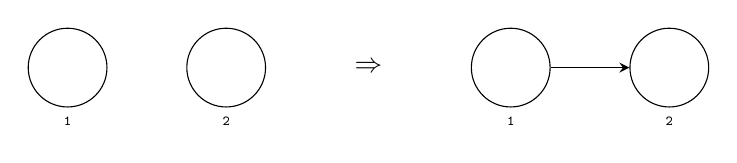
\begin{tikzpicture}

                \node         (transition) {$\Rightarrow$}            {};

                \node[vertex] (lhs 2) [label=below:\tiny{\texttt{2}},left=of transition]  {};
                \node[vertex] (lhs 1) [label=below:\tiny{\texttt{1}},left=of lhs 2]       {};

                \node[vertex] (rhs 1) [label=below:\tiny{\texttt{1}},right=of transition] {};
                \node[vertex] (rhs 2) [label=below:\tiny{\texttt{2}},right=of rhs 1]      {}
                    edge[post] (rhs 1);

            \end{tikzpicture}

            \\

            \texttt{where not edge(1, 2)}

        \end{tabular}
    \end{nscenter}
    \end{framed}
    \caption{A rule in GP2}
    \label{fig:RuleInGP2}
\end{figure}

Rules are the basic building blocks of a GP2 program and are defined by a
left-hand-side (LHS), a right-hand-side (RHS), and optionally a conditional
clause. A rule can be thought of as the definition of a transformation; a subgraph
matching the LHS of the rule is transformed to resemble the RHS. An example of a
GP2 rule is shown in \autoref{fig:RuleInGP2}.

The conditional clause is used to specify additional constraints on the subgraph
matching the LHS. Any match has to both match the LHS and conform to the constraints
defined by the conditional clause.

In a compiled program, a rule is split into two phases. The \emph{match} phase
searches the current graph for a subgraph which matches the LHS of the rule. This must
be an \emph{injective match}, meaning that each item in the LHS must be matched with
exactly one item in the host graph.

In this implementation of GP2, rule matches are chosen determinstically due to the
impracticality of generating all non-deterministic possibilities, which is what GP1 did.
If no match is found for the LHS, the rule is considered \emph{failed}. If a match is
found, the program moves on to the second phase, the \emph{application}.

A rule specifies a number of \emph{interface nodes}, nodes which are present in both
the LHS and the RHS. These interface nodes can be seen in \autoref{fig:RuleInGP2}; they
are the nodes with small numeric identifers below them. During the application phase,
any nodes in the LHS which are \emph{not} interface nodes will be deleted. Similarly,
any non-interface nodes which appear in the RHS will be created. At the end of the
application phase, the subgraph will match the RHS of the rule definition. The new
graph created by the application of this rule, an \emph{intermediate graph}, is then
used as the input to the next part of the program.

In the example in \autoref{fig:RuleInGP2}, the program will search for a subgraph
containing two nodes without an edge connecting them. If a match is found, it will
be transformed to resemble the RHS by adding an edge between the nodes.

%------------------------------------------------------------------------------

\subsubsection{Labels}
\label{sec:Labels}

Nodes and edges in a graph defined in GP2 can also have \emph{labels}. Labels
can be used cosmetically, without affecting the execution of the program, or
they can be included in rules to have the program read and modify labels.

\begin{figure}
    \begin{framed}
    \begin{nscenter}
        \begin{tikzpicture}
            \node (list) {\texttt{list}} {};
            \node (ss1)  [below=1mm of list] {\rotatebox{90}{$\subseteq$}} {};
            \node (atom) [below=1mm of ss1]  {\texttt{atom}} {};
            \node (ss2)  [below left=1mm of atom] {\rotatebox{45}{$\subseteq$}} {};
            \node (ss3)  [below right=1mm of atom] {\rotatebox{135}{$\subseteq$}} {};
            \node (int)  [below left=1mm of ss2] {\texttt{int}} {};
            \node (string) [below right=1mm of ss3] {\texttt{string}} {};
            \node (ss4)  [below=1mm of string] {\rotatebox{90}{$\subseteq$}} {};
            \node (char) [below=1mm of ss4] {\texttt{char}} {};

        \end{tikzpicture}
    \end{nscenter}
    \end{framed}
    \caption{GP2's type hierarchy for labels}
    \label{fig:TypeHierarchy}
\end{figure}

GP2 has a type hierarchy for labels, shown in \autoref{fig:TypeHierarchy}. Labels
can be of any of these five types. An \texttt{atom} consists of a single entity,
either an \texttt{int} or a \texttt{string}. A \texttt{list} is a collection of
zero or more \texttt{atom}s concatenated together; the concatenation is shown using
a colon (\texttt{:}).

Host graphs and the LHS and RHS of rules must be \emph{totally labelled}, meaning
that every node and edge must have a label. If the programmer wishes to use a node
or edge which appears to be unlabelled, they can use the empty list for that label.

Labels behave in two subtly different ways depending on where they are used. In a
graph, a label has a specific value, similar to an integer or string literal in a
convential programming language. When used in a rule, labels can either use literal
values to match nodes with exact label values, or they can use expressions which
can match a range of label values.

When matching a rule involving labels, GP2 finds a variable assignment which
matches the expressions of the labels in the graph. The values in this assignment
are identical when used in the RHS of the rule.

When using labels in a rule, the type of each label must be specified so that GP2
can find an assignment for each one. A rule which specifies a certain label type
can match any label with that type or a more specific type in the type hierarchy.
For example, a rule which contains a label of type \texttt{string} can match a
node which has a \texttt{char} label. The \texttt{list} type will match any label.

\begin{figure}
    \begin{framed}
    \begin{nscenter}
        \begin{tabular}{l}
            
            \texttt{swap(x, y: int)}

            \\

            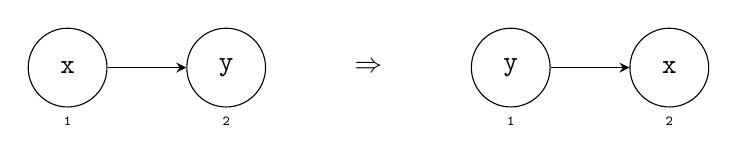
\begin{tikzpicture}

                \node         (transition) {$\Rightarrow$}            {};

                \node[vertex] (lhs 2) [label=below:\tiny{\texttt{2}},left=of transition]  {\texttt{y}}{};
                \node[vertex] (lhs 1) [label=below:\tiny{\texttt{1}},left=of lhs 2]       {\texttt{x}}{}
                    edge[pre] (lhs 2);

                \node[vertex] (rhs 1) [label=below:\tiny{\texttt{1}},right=of transition] {\texttt{y}}{};
                \node[vertex] (rhs 2) [label=below:\tiny{\texttt{2}},right=of rhs 1]      {\texttt{x}}{}
                    edge[post] (rhs 1);

            \end{tikzpicture}

            \\

            \texttt{where x > y}

        \end{tabular}
    \end{nscenter}
    \end{framed}
    \caption{A GP2 rule which uses labels}
    \label{fig:ExampleRuleWithLabels}
\end{figure}

The rule in \autoref{fig:ExampleRuleWithLabels} will only match a pair
of nodes where the labels are both integers, and the value of the source node's
label is greater than the value of the target node's label. This rule
demonstrates both that labels can be used as conditions in the program, and also
that a rule can modify labels. It also shows that labels act like variables when
used in a rule, since the values of \texttt{x} and \texttt{y} are re-used in the
RHS.

%------------------------------------------------------------------------------

\subsubsection{The Dangling Condition}
\label{sec:TheDanglingCondition}

\begin{figure}
\begin{framed}
    \begin{nscenter}
        \begin{tabular}{l}

            \texttt{delete(x, y, z: list)}

            \\

            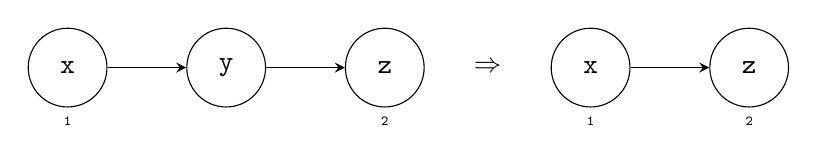
\begin{tikzpicture}

                \node         (transition) {$\Rightarrow$}            {};

                \node[vertex] (lhs 3) [label=below:\tiny{\texttt{2}},left=5mm of transition] {\texttt{z}} {};
                \node[vertex] (lhs 2) [left=of lhs 3]                                        {\texttt{y}} {}
                    edge[pre] (lhs 3);
                \node[vertex] (lhs 1) [label=below:\tiny{\texttt{1}},left=of lhs 2]          {\texttt{x}} {}
                    edge[pre] (lhs 2);

                \node[vertex] (rhs 1) [label=below:\tiny{\texttt{1}},right=5mm of transition] {\texttt{x}} {};
                \node[vertex] (rhs 2) [label=below:\tiny{\texttt{2}},right=of rhs 1]          {\texttt{z}} {}
                    edge[post] (rhs 1);

            \end{tikzpicture}

            \\\\\\

            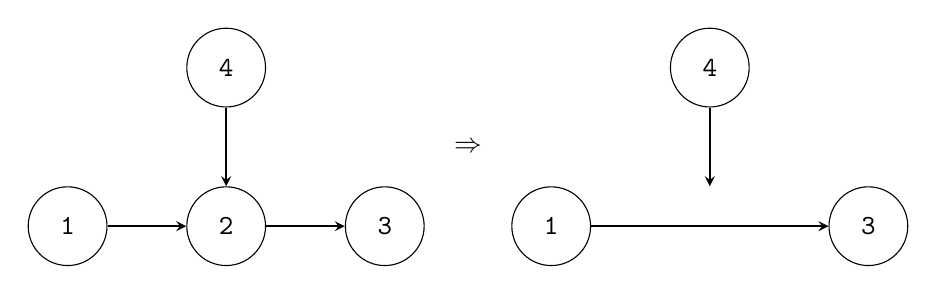
\begin{tikzpicture}

                \node (transition) {$\Rightarrow$} {};

                \node[vertex] (lhs c) [left=2.5mm of transition, yshift=-10mm] {\texttt{3}} {};
                \node[vertex] (lhs b) [left=of lhs c]                        {\texttt{2}} {}
                    edge[pre] (lhs c);
                \node[vertex] (lhs a) [left=of lhs b]                        {\texttt{1}} {}
                    edge[pre] (lhs b);
                \node[vertex] (lhs d) [above=of lhs b]                       {\texttt{4}} {}
                    edge[pre] (lhs b);


                \node[vertex]     (rhs a)         [right=2.5mm of transition, yshift=-10mm] {\texttt{1}} {};
                \node[invisible]  (rhs invisible) [right=of rhs a]                                     {};
                \node[vertex]     (rhs c)         [right=of rhs invisible]                {\texttt{3}} {}
                    edge[post]    (rhs a);
                \node[vertex]     (rhs d)         [above=of rhs invisible]                {\texttt{4}} {}
                    edge[pre]     (rhs invisible);

            \end{tikzpicture}

        \end{tabular}
    \end{nscenter}
    \end{framed}
    \caption{Attempting to apply a rule when the match violates the dangling condition}
    \label{fig:FailDanglingCondition}
\end{figure}

There is an additional condition which determines whether a rule can be matched, the
\emph{dangling condition}. This condition states that if a rule causes a node to be
deleted, the rule must also delete all edges incident to that node. In
other words, all non-interface nodes in a rule match must have no incoming or outgoing
edges which are not also part of the match.

\autoref{fig:FailDanglingCondition} shows the result of attempting to apply a rule
where the match violates the dangling condition. Since node 2 is not an interface
node, it is deleted during the application of the \texttt{delete} rule. However, the
rule does not specify that the edge from 4 to 2 should be deleted. This leaves a
\emph{dangling edge} from node 4 with no target. The dangling condition is used to
ensure that rule applications result in no dangling edges.

%------------------------------------------------------------------------------

\subsubsection{Programs}
\label{sec:Programs}

A GP2 program defines the order in which to apply rules using 8 simple control
structures:

\begin{description}
    \item[\textsc{Sequence}]
    Two subprograms separated by a semicolon ``\texttt{P; Q}'' are applied
    one after the other.

    \item[\textsc{Rule Set}]
    Rules in curly braces ``\texttt{\{R$_{\text{1}}$, R$_{\text{2}}$, R$_{\text{3}}$\}}''
    define a set, where exactly one rule from the set is executed, chosen
    non-determinstically from all rules in the set which have a valid match.
    If there are no rules in the set which match, the program fails in the
    same way as if a single rule failed to match.

    \item[\textsc{If-Then-Else}]
    In the statement ``\texttt{if C then P else Q}'', a copy of the graph is taken,
    before executing the sub-program \texttt{C}. The result, i.e. success or failure,
    is then used to determine whether to run \texttt{P} or \texttt{Q}. If C succeeded,
    \texttt{P} is executed on the copy of the original graph. If it failed, then
    \texttt{Q} is executed on the original graph. Note that by taking a copy first,
    any changes made by \texttt{C} are always reverted before executing either
    \texttt{P} or \texttt{Q}.

    \item[\textsc{Try-Then-Else}]
    Similar to \textsc{If-Then-Else}, but \texttt{C} is only reverted if it fails.
    Thus any changes made by \texttt{C} are \emph{not} reverted before executing
    \texttt{P}, but they \emph{are} reverted before executing \texttt{Q}.

    \item[\textsc{As-Long-As-Possible}]
    A subprogram followed by an exclamation point ``\texttt{P!}'' is executed
    repeatedly until it fails. When \texttt{P} fails, the graph is reverted back
    to the last successful state, that is, the state it was in at the end of the
    last successfully applied rule from \texttt{P}.

    The keyword \texttt{break} can also be used to exit from a loop before reaching
    the end. When using \texttt{break}, the graph is \emph{not} reverted before
    continuing with the program.

    \item[\textsc{Procedure}]
    Similar to a C preprocessor macro, a procedure is simply a named subprogram
    where any reference to the procedure name can be replaced with the definition
    of the procedure. Procedures are not allowed to be recursive.

    \item[\textsc{Skip}]
    A no-op which always succeeds, and does not affect the graph. Invoked using the
    keyword ``\texttt{skip}''. This is the same as executing a rule with an empty
    LHS and an empty RHS, which always matches and does nothing to the graph.

    \item[\textsc{Fail}]
    A statement which always fails and does not affect the graph. This is the same
    as attempting to execute a rule for which there are no matches. Invoked using
    the keyword ``\texttt{fail}''. It can also be simulated using an empty
    \textsc{Rule Set} \texttt{\{\}}.

    \item[\textsc{Or}]
    In the statement ''\texttt{P or Q}'', exactly one subprogram, either \texttt{P}
    or \texttt{Q} is chosen non-deterministically and executed. Unlike the
    \textsc{Rule Set} construction, if the chosen subprogram fails, the other is
    \emph{not} applied instead, and the program fails.
\end{description}

For GP2, a subprogram is either a single rule, referenced by its name, or one of
the above control structures. Therefore it is possible to nest control structures
to create more complex programs.

In general, execution of a program continues until either all statements are
executed, or until a statement results in an attempt to apply a rule which has
no matches in the graph. The exceptions to this are \textsc{As-Long-As-Possible}
statements, and the conditional statements in \textsc{If-Then-Else} and
\textsc{Try-Then-Else} structures. In these cases, a failure to match a rule
does not halt execution of the program.

\autoref{fig:ExampleProgramDefinition} shows an example GP2 program, an adapted
version of the program used as a case study in Bak's thesis on GP2 \citep[p.126]{bak2015}.
It is a simple program which determines whether a graph is \emph{2-colourable},
that is, its nodes can be coloured using two different colours without two nodes
of the same colour being connected by an edge. This program requires that the
graph is \emph{connected}, meaning there is an undirected path between every pair
of nodes.

This program consists of four rules and uses many of the constructs outlined
previously, including \textsc{Try-Then-Else}, \textsc{If-Then-Else},
\textsc{Rule Set}s, \textsc{As-Long-As-Possible} and \textsc{Procedure}s.

It also takes advantage of another feature of GP2, the ability to \emph{colour}
a node. The colour of a node is a property which can be set by a rule, or the
host graph can contain coloured nodes. The colour is taken into account when
searching for a rule match; for example, in this program, \texttt{joined\_reds}
will only match when both the nodes' colours are red.

\begin{figure}[!htb]
\begin{framed}
    \begin{nscenter}
        \begin{verbatim}
Main = try (init; Colour!; if Invalid then fail)
Colour = {colour_blue, colour_red}
Invalid = {joined_reds, joined_blues}
        \end{verbatim}

        \begin{tabular}{l}            

            \texttt{init}

            \\ 

            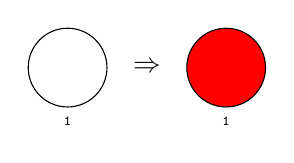
\begin{tikzpicture}

                \node         (transition) {$\Rightarrow$}                                       {};

                \node[vertex] (lhs) [label=below:\tiny{\texttt{1}},left=2mm of transition]           {};

                \node[vertex] (rhs) [label=below:\tiny{\texttt{1}},right=2mm of transition,fill=red] {};

            \end{tikzpicture}

            \\\\

            \texttt{joined\_reds}

            \\

            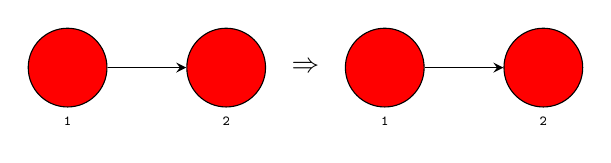
\begin{tikzpicture}

                \node         (transition) {$\Rightarrow$}                                         {};

                \node[vertex] (lhs 2) [label=below:\tiny{\texttt{2}},left=2mm of transition,fill=red]  {};
                \node[vertex] (lhs 1) [label=below:\tiny{\texttt{1}},left=of lhs 2,fill=red]       {}
                    edge[pre] (lhs 2);

                \node[vertex] (rhs 1) [label=below:\tiny{\texttt{1}},right=2mm of transition,fill=red] {};
                \node[vertex] (rhs 2) [label=below:\tiny{\texttt{2}},right=of rhs 1,fill=red]      {}
                    edge[post] (rhs 1);

            \end{tikzpicture}

            \\\\

            \texttt{joined\_blues}

            \\

            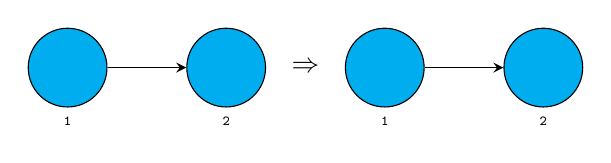
\begin{tikzpicture}

                \node         (transition) {$\Rightarrow$}                                          {};

                \node[vertex] (lhs 2) [label=below:\tiny{\texttt{2}},left=2mm of transition,fill=cyan]  {};
                \node[vertex] (lhs 1) [label=below:\tiny{\texttt{1}},left=of lhs 2,fill=cyan]       {}
                    edge[pre] (lhs 2);

                \node[vertex] (rhs 1) [label=below:\tiny{\texttt{1}},right=2mm of transition,fill=cyan] {};
                \node[vertex] (rhs 2) [label=below:\tiny{\texttt{2}},right=of rhs 1,fill=cyan]      {}
                    edge[post] (rhs 1);

            \end{tikzpicture}

            \\\\

            \texttt{colour\_blue}

            \\

            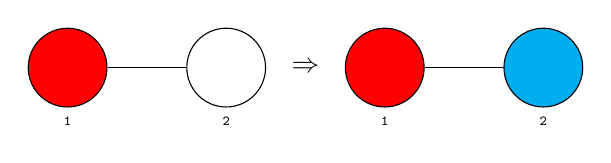
\begin{tikzpicture}

                \node         (transition) {$\Rightarrow$}                                          {};

                \node[vertex] (lhs 2) [label=below:\tiny{\texttt{2}},left=2mm of transition]            {};
                \node[vertex] (lhs 1) [label=below:\tiny{\texttt{1}},left=of lhs 2,fill=red]        {}
                    edge[bi] (lhs 2);

                \node[vertex] (rhs 1) [label=below:\tiny{\texttt{1}},right=2mm of transition,fill=red]  {};
                \node[vertex] (rhs 2) [label=below:\tiny{\texttt{2}},right=of rhs 1,fill=cyan]      {}
                    edge[bi] (rhs 1);

            \end{tikzpicture}

            \\\\

            \texttt{colour\_red}

            \\

            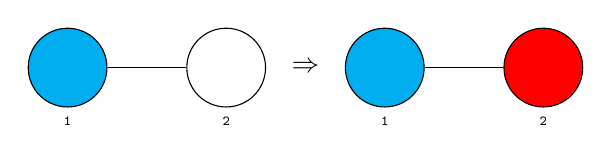
\begin{tikzpicture}

                \node         (transition) {$\Rightarrow$}                                          {};

                \node[vertex] (lhs 2) [label=below:\tiny{\texttt{2}},left=2mm of transition]            {};
                \node[vertex] (lhs 1) [label=below:\tiny{\texttt{1}},left=of lhs 2,fill=cyan]       {}
                    edge[bi] (lhs 2);

                \node[vertex] (rhs 1) [label=below:\tiny{\texttt{1}},right=2mm of transition,fill=cyan] {};
                \node[vertex] (rhs 2) [label=below:\tiny{\texttt{2}},right=of rhs 1,fill=red]       {}
                    edge[bi] (rhs 1);

            \end{tikzpicture}

        \end{tabular}
    \end{nscenter}
    \end{framed}
    \caption{Definition of 2-colouring in GP2}
    \label{fig:ExampleProgramDefinition}
\end{figure}

\begin{figure}
    \begin{framed}
    \begin{nscenter}
        \begin{tabular}{l}    

            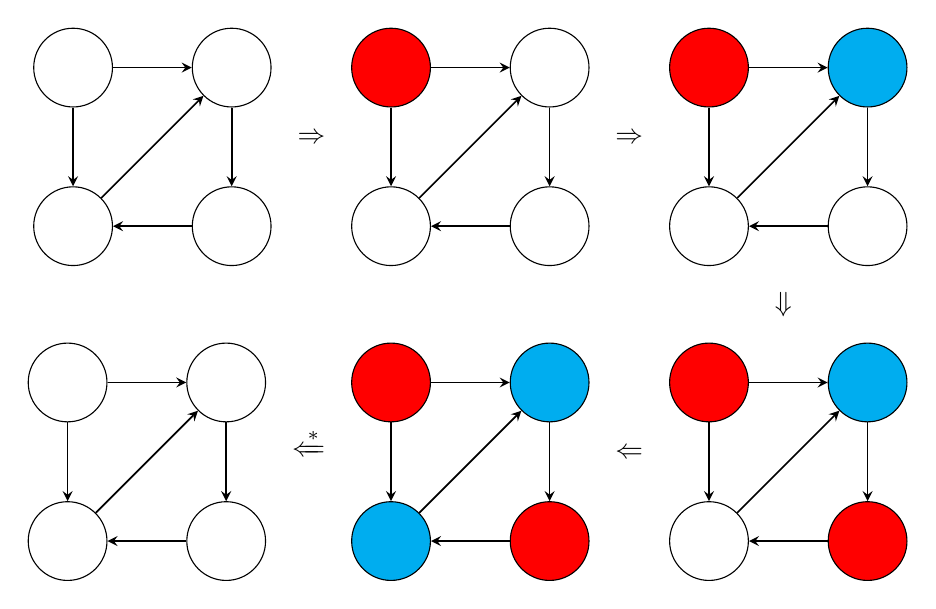
\begin{tikzpicture}
                [vertex/.style={circle,draw,minimum size=10mm}]

                \node (transition1) {$\Rightarrow$} {};

                \node[vertex]  (12) [above left=5mm of transition1] {};
                \node[vertex]  (13) [below=of 12]               {}
                    edge[post] (12);
                \node[vertex]  (11) [left=of 12]                {}
                    edge[pre]  (12);
                \node[vertex]  (14) [below=of 11]               {}
                    edge[post] (11)
                    edge[pre]  (12)
                    edge[post] (13);

                \node[vertex]  (21) [above right=5mm of transition1,fill=red] {};
                \node[vertex]  (22) [right=of 21]                         {}
                    edge[post] (21);
                \node[vertex]  (23) [below=of 22]                         {}
                    edge[post] (22);
                \node[vertex]  (24) [below=of 21]                         {}
                    edge[post] (21)
                    edge[pre]  (22)
                    edge[post] (23);

                \node (transition2) [below right=5mm of 22] {$\Rightarrow$} {};

                \node[vertex]  (31) [above right=5mm of transition2,fill=red] {};
                \node[vertex]  (32) [right=of 31,fill=cyan]               {}
                    edge[post] (31);
                \node[vertex]  (33) [below=of 32]                         {}
                    edge[post] (32);
                \node[vertex]  (34) [below=of 31]                         {}
                    edge[post] (31)
                    edge[pre]  (32)
                    edge[post] (33);

                \node (transition3) [below right=5mm of 34] {$\Downarrow$} {};

                \node[vertex]  (41) [below left=5mm of transition3,fill=red] {};
                \node[vertex]  (42) [right=of 41,fill=cyan]                  {}
                    edge[post] (41);
                \node[vertex]  (43) [below=of 42,fill=red]                   {}
                    edge[post] (42);
                \node[vertex]  (44) [below=of 41]                            {}
                    edge[post] (41)
                    edge[pre]  (42)
                    edge[post] (43);

                \node (transition4) [below left=5mm of 41] {$\Leftarrow$} {};

                \node[vertex]  (52) [above left=5mm of transition4,fill=cyan] {};
                \node[vertex]  (51) [left=of 52,fill=red]                   {}
                    edge[pre]  (52);
                \node[vertex]  (53) [below=of 52,fill=red]                  {}
                    edge[post] (52);
                \node[vertex]  (54) [below=of 51,fill=cyan]                  {}
                    edge[post] (51)
                    edge[pre]  (52)
                    edge[post] (53);

                \node (transition5) [below left=5mm of 51, yshift=2.5mm] {$\xLeftarrow{*}$} {};

                \node[vertex]  (62) [above left=5mm of transition5, yshift=-2.5mm] {};
                \node[vertex]  (61) [left=of 62]                    {}
                    edge[pre]  (62);
                \node[vertex]  (63) [below=of 62]                   {}
                    edge[post] (62);
                \node[vertex]  (64) [below=of 61]                   {}
                    edge[post] (61)
                    edge[pre]  (62)
                    edge[post] (63);

            \end{tikzpicture}

        \end{tabular}
    \end{nscenter}
    \end{framed}
    \caption{Example execution of 2-colouring}
    \label{fig:ExampleProgramExecution}
\end{figure}

An example execution of the 2-colouring program is shown in \autoref{fig:ExampleProgramExecution}.
Starting with an uncoloured graph, the algorithm picks a node and colours it red
using the \texttt{init} rule. It then traverses the graph colouring nodes in
alternating colours using the \texttt{colour\_blue} and \texttt{colour\_red} rules,
by defining them as a \textsc{Rule Set} in a \textsc{Procedure} and executing
it \textsc{As-Long-As-Possible}. When no more uncoloured nodes are present in the
graph, the \texttt{Colour} procedure will be unable to match any further rules,
so it will end.

To check whether the produced colouring is valid, the entire \texttt{Main}
procedure is wrapped in a \textsc{Try-Then-Else} statement. After executing
\texttt{Colour}, the \texttt{Invalid} procedure runs. This procedure uses the
two remaining rules, \texttt{joined\_reds} and \texttt{joined\_blues}, to see if
any adjacent nodes are the same colour. If they are, one of these rules will
match, triggering the conditional statement \texttt{fail} from the
\textsc{If-Then-Else} statement. This in turn causes the outer \texttt{try} to
fail, reverting all changes made to the graph and returning the uncoloured input
graph.

However, if \texttt{Invalid} fails to match either of the rules, it must mean
that no two same-coloured nodes are connected via an edge. This means that it is
a valid colouring. The \texttt{fail} statement is not executed, meaning the
\texttt{try} succeeds. The changes to the graph are kept, and the modified graph
is returned as the result of the program.

In the example execution in \autoref{fig:ExampleProgramExecution}, the host graph
is not 2-colourable. When the rules in \texttt{Colour} can no longer be matched,
\texttt{joined\_blues} inside \texttt{Invalid} will match with the nodes in the
bottom-left and top-right of the graph. Because this rule was successfully applied
(even though it has no effect on the graph), the \textsc{If-Then-Else} causes the
program to enter the fail state. This in turn means that the \textsc{Try-Then-Else}
surrounding the program fails, and all the changes made to the input graph are
reversed. The output graph is therefore identical to the input graph.

%//////////////////////////////////////////////////////////////////////////////

\section{Tracing and Debugging}
\label{sec:TracingAndDebugging}

\subsection{Debugging in Imperative Languages}
\label{sec:DebuggingInImperativeLanguages}

When programming in a high level imperative language, such as C or Java, the
programmer will more often than not have access to a \emph{debugger}. In
\citep{sammet1969}, Sammet says that a program in a high level language without
debugger support may be ''harder to debug than an assembly language which the
programmer understands'', since the programmer has to interpret the compiled code,
rather than reading the source code they wrote.

Most language interpreters and Integrated Development Environments (IDEs) have a
debugger built in \citep{scott2009}, and standalone debuggers are also available
for some languages. For C, this may be \texttt{gdb} \citep{gdbsite}, while for
Java, it might be \texttt{jdb} \citep{jdbsite}. 

A debugger is intended to allow the programmer to pause their program during
execution, so that they can inspect the contents of variables and other memory
locations. It also allows them to run their program step-by-step to see its
execution flow; they may wish to check that a function is called at the expected
point during execution, for instance.

Some debuggers also include more advanced features to make debugging easier and to
give the programmer more insight into their program. Breakpoints are a common feature
which allow the programmer to specify a line of source code and have the program
execute normally until the breakpoint is reached, at which point execution will
pause, or \emph{break}.

Because GP2 has a rule-based structure, unlike imperative programming languages,
it is not clear what a ''line of code'' represents in a GP2 program. The textual
part of a GP2 program can indeed have lines, but since a single line in a GP2
program can be complex and use many rules, this is too high-level to consider a
''line of code'' as a debugger does. In an imperative language, a single line of
code may only perform one or two actions, so inspecting each line individually
shows the flow of the program. In GP2, running a line of the textual program
could result in tens or hundreds of rules being applied if \textsc{As-Long-As-Possible}
is used, for example. It may be inappropriate to focus on how debuggers are
implemented for imperative languages when considering GP2.

%------------------------------------------------------------------------------

\subsubsection{IDEs}
\label{sec:IDEs}

A debugger is often available from within the Integrated Development Environment
(IDE) for a language. For example, the Visual Studio IDE for C, C++, and C\#
includes the Visual Studio Debugger \citep{msdnsite}. One of the most prevalent
Java IDEs, Eclipse, integrates with \texttt{jdb} \citep{eclipsesite}.

When an IDE integrates with a debugger, it can provide additional functionality
by allowing the programmer to interact with the source code and the debugger
visually in the same environment. Visual Studio and Eclipse both allow breakpoints
to be set directly on a line of source code in the editor, for instance. IDEs
often allow the programmer to trace program execution through the source code,
by highlighting each line of code as the programmer steps through in the debugger.

It may be useful to use some of these ideas for GP2. For instance, when stepping
through a GP2 program, it would be helpful to highlight the current statement or
rule being executed, to give the user context.

%------------------------------------------------------------------------------

\subsubsection{Edit-and-Continue}
\label{sec:EditAndContinue}

Edit-and-continue is an even more advanced feature which requires specific
compiler support, and is usually only available in IDEs, since they have access
to both the compiler and the debugger. It allows the programmer to pause execution
of the program, edit the source code, recompile the program, and continue execution
from the previous paused state, without having to restart the program from the
beginning. Edit-and-continue is useful for reducing the time taken to find and
fix bugs, since fixes can be implemented and tested without having to stop and
restart the program's execution.

It is unclear whether edit-and-continue would be a good addition to GP2. On one
hand, it can speed up debugging because the programmer does not have to start the
program again from the beginning. On the other hand, it is not clear how this
feature could be implemented in GP2. It would not make sense for the user to be
able to edit the input graph or an intermediate graph while execution is paused,
because the result of the program would be incorrect. Editing the rules and
program text would make more sense, but this could lead to problems, such as if
the user pauses execution after matching a rule, and then edits that rule in
a way that makes the match incorrect.

%------------------------------------------------------------------------------

\subsubsection{Reverse Debugging}
\label{sec:ReverseDebugging}

\texttt{gdb} supports what is called \emph{reverse debugging} \citep{gdbreversesite}.
This allows program execution to actually be reversed, running the program
backwards to reach an earlier state. This can come in useful to look for
non-deterministic bugs which do not always occur; the program can be run until
the bug occurs, then executed in reverse to look for the cause.

This ability comes with a trade-off, however; running with reverse debugging
enabled reduces the performance of the running program. It can only be used in
specific cases and cannot be enabled all the time, since the program would run
much slower and possibly exhibit time-related bugs. Reverse debugging is also
only available for \texttt{gdb} running on Linux.

\texttt{gdb}'s implementation of reverse debugging involves recording the machine
state after each instruction exectuion, including the values stored in memory and
registers. To reverse an instruction, the state from the previous instruction is
simply restored, making it appear as if the reversed instruction was never
executed. This implementation allows powerful interaction with the program; it
can reverse a single instruction at a time, or it can be run backwards until a
breakpoint is reached. In theory, although \texttt{gdb} does not support this,
this system could allow a form of ''checkpointing'' where execution can be skipped
directly back to an arbitrary point by simply restoring the state from that point.

Reverse debugging may be a useful feature for GP2, because it would allow a
programmer to step backwards through the execution of a GP2 program to inspect
the intermediate graph before and after a rule application, to see what changed.
This method is more akin to tracing than traditional debugging, since the debugger
is storing a history of everything that occurs during execution.

While the implementation of reverse debugging in \texttt{gdb} is limited to the
Linux platform, this is because its implementation requires monitoring calls to
the kernel and system APIs. This is irrelevant to GP2, because it would only
need to trace rule matches and applications, both of which are implemented inside
GP2 itself.

%==============================================================================

\subsection{Tracing in Functional Languages}
\label{sec:TracingInFunctionalLanguages}

The syntax and execution of a GP2 program is very similar to that of a functional
programming language. For example, a function in Haskell is similar to a rule or
set of rules in GP2; the function defines left-hand-sides and right-hand-sides,
and executing it with an argument looks for a LHS which matches the argument,
and returns the RHS. This similarity to the matching and application of rules in
GP2 suggests that it would be appropriate to consider it like a functional
language when implementing debugging or tracing.

Because of the nature of functional languages, it is rare to see traditional
debuggers like those used with imperative languages \citep{wadler1998}. Lazy
evaluation, where the value of a statement is only calculated when it is required,
means that pausing execution on a line of code may not reveal the value of a
statement on that line, because it will not be evaluated until later in the program.

To avoid this problem, functional programmers will often use tracing instead.
This is where additional code is added to the program which simply outputs
information about what the program is doing, either to the console or to a file on
disk. The progammer then reads this information back once the program has finished,
to see what steps the program took and identify where it differed from the
expected execution.

Tracing can be done in primitive ways, by manually adding \texttt{print}
statements to the code, but there are also more sophisticated tools available.
For Haskell, for instance, a handful of different tracing tools are
available \citep{runciman2000}. Two of them, Freja and Hat, are modified Haskell
compilers which add automatic tracing functionality to the compiled program. When
the program runs, trace information is stored in the program heap, which can then
be accessed at the end of execution. The other tool, Hood, is a Haskell library
which is used by importing it and adding \texttt{observe} annotations to the code,
which preserve lazy evaluation and output information about the program as it runs.
The programmer would then inspect the output from the annotations to trace through
the program.

The benefit of compiler based tools like Freja and Hat is the programmer does not
need to think about where to put tracing code, since all code is traced automatically
in the compiled program. However, storing a full trace of an entire program takes
up space either in memory or on disk; the advantage of a manual tool like Hood is
the programmer can reduce the number of trace points to reduce the trace size.

Another disadvantage of Hat is that it has a very large impact on performance,
running more than ten times slower than the original Haskell program \citep{runciman2000}.
Hat adds a lot of overhead at runtime, since the program has to do a lot of
extra work to store the tracing data. On the other hand, Freja is also a tracing
tool, yet Chitil, Runciman, and Koopman state that the overhead is ''not
noticeable''. It is clear that the performance impact of these tools depends on
their implementation.

%==============================================================================

\subsection{Debugging With Other Graph Programming Tools}
\label{sec:DebuggingOtherGraphProgrammingTools}

Each of the three other graph programming tools mentioned in
Section~\ref{sec:GraphProgramming} have their own debugging or tracing tools.

\subsubsection{AGG}

Of the three tools, AGG has the simplest debugging tools. It allows the user to
select a rule in their graph grammar and then look through all the matches for
that rule, by showing them on the current graph.

A unique feature of AGG is that it also allows the user to manually create a
match; by selecting nodes and edges first in the LHS of the rule, and then in
the graph, the user creates a mapping between the rule and the current graph to
create a match. The tool will alert the user if they attempt to select a mapping
which is not a true match.

When a match has been chosen, either automatically or manually, the rule can then
be applied by clicking a \texttt{Transformation Step} button in the editor. After
a rule has been applied, an \texttt{Undo Step} button becomes available which
reverts the changes made by the most recent rule application.

\subsubsection{GROOVE}

GROOVE also allows the user to inspect all possible rule matches for the current
graph. In the list of rules shown in the editor, the possible matches for each are
shown underneath each rule. These matches can be clicked to highlight them on the
graph, and double-clicking applies the rule, updating the graph.

Similar to AGG, it is possible to undo a single rule application. However, GROOVE
also keeps a history of all previous graph states. In the ''State Space Explorer'',
the tool shows a transition diagram containing all the previously visited graph
states, with the transitions representing the rule applied to reach a given state.
In this view, the user can select a previous state and jump back to it, allowing
the user to undo multiple rule applications at once, or even undoing previous rule
applications and re-applying other rules, in one step.

\subsubsection{GrGen}

GrGen's debugger is different in that it is controlled using a command-line style
interface, rather than using buttons in the editor UI. It provides a command to
apply a single rule, similar to the other two tools.

However, when applying a rule, GrGen can show more detail. It can show the steps
required to apply a rule: the match, the modification to the graph, and the result.
It shows each of these stages individually, highlighting the relevant areas on the
graph at each stage.

Another unique feature of GrGen's debugger is that it allows the user to tell the
program to run until the end of the current loop. GrGen supports a loop structure
similar to GP2's \textsc{As-Long-As-Possible}, and the debugger's \texttt{step out}
command will continue to execute until the current loop ends, giving control back
to the user.

Finally, GrGren also supports a feature similar to breakpoints. It allows the user
to specify a condition, and when that condition is met, execution will pause. One
type of condition which can be specified is a certain modification to the graph,
such as pausing execution when a specific node is deleted from the graph.

%==============================================================================

\subsection{Previous Work on Debugging in GP2}
\label{sec:PreviousWorkOnDebuggingInGP2}

There has been some previous work to add debugging facilities to GP2 \citep{taylor2016}.
This work was focused on modifying the compiler to support stepping through a
program.

In that project, command-line arguments were added to allow the user to specify
how big a ''step'' should be, and how many steps to execute before stopping.
This allows GP2 to approximate breakpoints by picking an appropriate step size
and count in order to finish execution at the point the programmer is interested in.

However, there are some problems with this method. For one, once the specified
number of steps have been executed, the program terminates completely and outputs
the current graph. This means that if the programmer wishes to step through the
program one rule at a time, for example, they must run the compiler multiple times
and increase the number of steps by one each time, wasting time by re-executing
earlier steps at each iteration.

Another problem is that, although the compiler was modified, the graphical editor
remains unchanged, and so does not support the new partial execution feature.
For the feature to be most useful, it would have to be integrated into the editor.


\clearpage

%XXXXXXXXXXXXXXXXXXXXXXXXXXXXXXXXXXXXXXXXXXXXXXXXXXXXXXXXXXXXXXXXXXXXXXXXXXXXXX

\chapter{Requirements}
\label{cha:Requirements}

Before designing and implementing a system, the requirements for the system need
to be considered. These requirements should be based on expected real-world usage
of the tool and keep the goals of the tool in mind.

\section{Potential Users}
\label{sec:Potential Users}

In order to decide what the requirements for a debugging tool are, it is useful
to consider the types of user who would potentially use such a tool. There are
two main potential audiences for a GP2 debugging tool:

\begin{itemize}
    \item Programmers who have written a GP2 program which they would like to
          debug. Either the program produces unexpected output, or it never
          terminates, so the programmer wishes to use the debugging tools to
          understand why their program is behaving incorrectly, and then fix the
          bug.

    \item New users of GP2 who are still learning the language. GP2 is an
          unconvential language and its concepts can be unfamiliar to
          inexperienced users. Allowing these users to step through a GP2
          program would let them see how GP2 works and help them to understand
          the language faster.

          However, it should be noted that the debugger is not a substitute for
          documentation or user manuals; the debugger should not be expected to
          explain the semantics of GP2, but rather act as a tool to show the
          process of running a GP2 program.
\end{itemize}

%//////////////////////////////////////////////////////////////////////////////

\section{Integration and Maintainability}
\label{sec:IntegrationAndMaintainability}

Consideration should also be given to how the new features are integrated into
GP2. The experience of using existing GP2 features should be unaffected, and the
codebase should stay maintainable for future developers of GP2. The high-level
requirements this leads to are:

\begin{itemize}
    \item Backwards compatibility. Adding a debugging tool should not impact the
          existing features of GP2, the compiler, or the IDE. Programs written
          before the addition of debugging tools should still be runnable in the
          new IDE.

    \item Make debugging optional. The user should not be forced to use the
          debugging tools every time they run their program, and should be able
          to choose when to enable them.

    \item Minimise the performance impact. Running a program with debugging tools
          should affect performance as little as possible, and running with
          debugging disabled should have no performance impact compared to the
          previous version of GP2.

    \item Keep the codebase maintainable. When modifying existing code, or adding
          new code, follow conventions and make code readable. Make the intent
          of any changes clear to ensure future developers will understand what
          has been changed.

    \item Consider dependencies between components. To implement debugging will
          require modifying both the compiler and the IDE. It is important to
          consider the dependencies between these components, to ensure that
          they can still function independently.

          It is also important to consider the dependencies between new code and
          existing code. If bugs are discovered in the compiler, for example, it
          must be possible to fix them without needing to modify the code added
          for debugging, and vice versa, since compilation and debugging should
          be separate components. Compilation should still work independently
          of debugging. 
\end{itemize}

%//////////////////////////////////////////////////////////////////////////////

\section{User Scenarios}
\label{sec:UserScenarios}

To further identify specific low level requirements for the tool, two
hypothetical user scenarios have been created to show potential situations a
user could be in, and how the debugging tools can help the user complete their
task in those situations.

%==============================================================================

\subsection{Experienced GP2 Programmer}

In the first scenario, the user is an experienced GP2 programmer who understands
all the concepts and semantics of GP2. They have written a program similar to
the one shown in \autoref{fig:ExampleProgramDefinition}, to determine whether a
graph is two-colourable.

However, their program is slightly different, and does not output the coloured
graph when it is two-colourable; instead, the original, uncoloured graph is
always returned, and an extra node is added to show the result. If the graph is
two-colourable, a green node is added, otherwise a red node is added. The
program they have written is shown in \autoref{fig:AlternateTwoColourableProgram},
along with the two new rules, \texttt{add\_red\_node} and \texttt{add\_green\_node}.
The other rules are omitted since they are identical to the rules in the
original program.

\begin{figure}
    \begin{framed}
        \begin{nscenter}
            \begin{verbatim}
Main = if (init; Colour!; Invalid)
           then add_red_node
           else add_green_node
Colour = {colour_blue, colour_red}
Invalid = {joined_blues, joined_blues}
            \end{verbatim}

            \begin{tabular}{l @{\hskip 20mm} l}
                \texttt{add\_red\_node} & \texttt{add\_green\_node}
                
                \\

                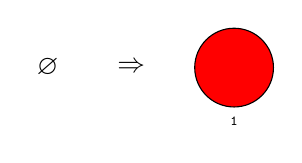
\begin{tikzpicture}
                    \node         (transition) {$\Rightarrow$}                                           {};
                    \node         (lhs) [left=5mm of transition] {$\varnothing$}                         {};
                    \node[vertex] (rhs) [label=below:\tiny{\texttt{1}},right=5mm of transition,fill=red] {};
                \end{tikzpicture}

                &

                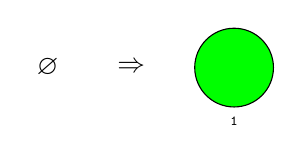
\begin{tikzpicture}
                    \node         (transition) {$\Rightarrow$}                                           {};
                    \node         (lhs) [left=5mm of transition] {$\varnothing$}                         {};
                    \node[vertex] (rhs) [label=below:\tiny{\texttt{1}},right=5mm of transition,fill=green] {};
                \end{tikzpicture}
            \end{tabular}
        \end{nscenter}
    \end{framed}
    \caption{Alternate version of the 2-colourable program}
    \label{fig:AlternateTwoColourableProgram}
\end{figure}

Unfortunately, when they test their program, for some inputs it gives the
incorrect result; for certain non-two-colourable graphs, the program still adds
a green node to indicate that it is two-colourable. Just by inspecting the
program, the user cannot determine what the bug is with the program, so they
decide to use the simplest possible non-two-colourable input graph, shown in
\autoref{fig:SimplestNonTwoColourableGraph}, and use the debugger to step
through their program.

\begin{figure}
    \begin{framed}
        \begin{nscenter}
            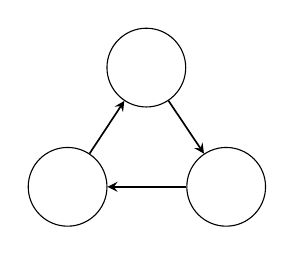
\begin{tikzpicture}
                \node[vertex] (top) {};
                \node[vertex] (left) [below=5mm of top, xshift=-10mm] {}
                    edge[pre] (top);
                \node[vertex] (right) [right=10mm of left] {}
                    edge[post] (top)
                    edge[pre] (left);
            \end{tikzpicture}
        \end{nscenter}
    \end{framed}
    \caption{Simplest possible non-two-colourable graph}
    \label{fig:SimplestNonTwoColourableGraph}
\end{figure}

As they step through the program, the \texttt{init} rule colours the top node red,
then \texttt{colour\_blue} is applied, followed by \texttt{colour\_red}. This results
in the graph being coloured red, blue, red running clockwise. Clearly the rules
for colouring nodes are defined correctly, so the bug must be in the error
detection logic.

They continue stepping through the program and it reaches the \texttt{Invalid}
procedure. They use the debugger to highlight a match for \texttt{Invalid}
without applying it, and it turns out there are none, which should not be the
case. They first look at the definitions for the \texttt{joined\_reds} and
\texttt{joined\_blues} rules, and they are definitely correct. Finally they look
at the definition of \texttt{Invalid} itself, and realise they have put
\texttt{joined\_blues} in the rule set twice, so \texttt{joined\_reds} is never
actually used.

The bug in this program was fairly subtle, since the general structure of the
program is mostly correct; there are two rules in \texttt{Invalid} as expected,
but the same rule was added twice. Without the debugger to step through the
program, it may have taken much longer to spot this mistake, since stepping
through allowed the user to see the coloured graph before it was reverted by
the \texttt{if} statement.

The ability to view a match without applying it also helped in this case, since
it allowed the user to see that none of the rules in \texttt{Invalid} matched,
without automatically exiting the \texttt{if} condition when no rules matched.

%==============================================================================

\subsection{New User Learning GP2}

In the second scenario, the user is inexperienced with GP2 and is still trying
to learn the language. They understand most of how the language works, but they
are having trouble with understanding the in semantics of \textsc{If-Then-Else}.

\begin{figure}[!htb]
    \begin{framed}
        \begin{nscenter}
            \begin{tabular}{l}
                \texttt{Main = if insert then bridge else loop}
                \\\\
                \texttt{insert}
                \\
                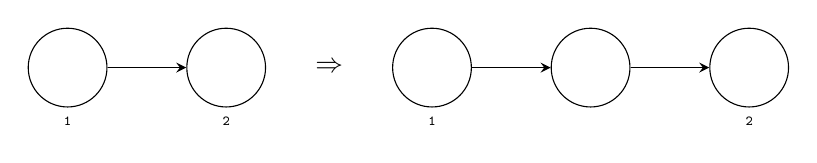
\begin{tikzpicture}
                    \node         (transition) {$\Rightarrow$}            {};

                    \node[vertex] (lhs 2) [label=below:\tiny{\texttt{2}},left=5mm of transition] {};
                    \node[vertex] (lhs 1) [label=below:\tiny{\texttt{1}},left=of lhs 2]          {}
                        edge[pre] (lhs 2);

                    \node[vertex] (rhs 1) [label=below:\tiny{\texttt{1}},right=5mm of transition] {};
                    \node[vertex] (rhs 2) [right=of rhs 1]                                        {}
                        edge[post] (rhs 1);
                    \node[vertex] (rhs 3) [label=below:\tiny{\texttt{2}}, right=of rhs 2]         {}
                        edge[post] (rhs 2);
                \end{tikzpicture}
                \\\\
                \texttt{bridge}
                \\
                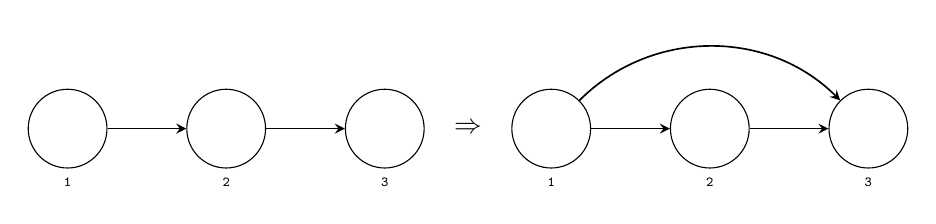
\begin{tikzpicture}
                   \node         (transition) {$\Rightarrow$}            {};

                    \node[vertex] (lhs 3) [label=below:\tiny{\texttt{3}},left=2.5mm of transition]   {};
                    \node[vertex] (lhs 2) [label=below:\tiny{\texttt{2}},left=of lhs 3]            {}
                        edge[pre] (lhs 3);
                    \node[vertex] (lhs 1) [label=below:\tiny{\texttt{1}},left=of lhs 2]            {}
                        edge[pre] (lhs 2);

                    \node[vertex] (rhs 1) [label=below:\tiny{\texttt{1}},right=2.5mm of transition]  {};
                    \node[vertex] (rhs 2) [label=below:\tiny{\texttt{2}},right=of rhs 1]           {}
                        edge[post] (rhs 1);
                    \node[vertex] (rhs 3) [label=below:\tiny{\texttt{3}},right=of rhs 2]           {}
                        edge[post] (rhs 2)
                        edge[post,bend right=45] (rhs 1);
                \end{tikzpicture}
                \\\\
                \texttt{loop}
                \\
                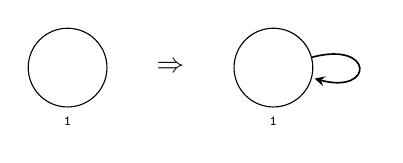
\begin{tikzpicture}
                    \node         (transition) {$\Rightarrow$}            {};

                    \node[vertex] (lhs 1) [label=below:\tiny{\texttt{1}},left=5mm of transition] {};

                    \node[vertex] (rhs 1) [label=below:\tiny{\texttt{1}},right=5mm of transition] {}
                        edge [post,loop right] (rhs 1);
                \end{tikzpicture}
                \\\\
                Input graph:
                \\\\
                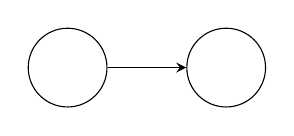
\begin{tikzpicture}
                    \node[vertex] (node 1) [yshift=5mm]                 {};
                    \node[vertex] (node 2) [right=of node 1] {}
                        edge[post] (node 1);
                \end{tikzpicture}
            \end{tabular}
        \end{nscenter}
    \end{framed}
    \caption{Simple program to learn the semantics of \textsc{If-Then-Else}}
    \label{fig:LearnSemanticsOfIf}
\end{figure}

They have written a very simple GP2 program, shown in \autoref{fig:LearnSemanticsOfIf},
which consists of three rules and a single \textsc{If-Then-Else} statement. When
they run this program on the input graph shown, they incorrectly expect the
output graph to match the RHS of the \texttt{bridge} rule, because they expect
\texttt{insert} to be applied, followed by \texttt{bridge}.

In actuality, this program fails, because the changes made by \texttt{insert}
are reverted before attempting to match \texttt{bridge}, meaning there is no
possible match for \texttt{bridge}.

The result confuses the user, who then decides to use the debugger to step
through the program to see what happened. The first thing they see is the
program tries to match \texttt{insert} and succeeds, which they expected.
However, then they advance to the next execution step and are surprised that
no changes have been made to the graph. They then realise that they had mixed
up the semantics of \textsc{If-Then-Else} and \textsc{Try-Then-Else}.

Ideally in this situation, the debugger would explicitly show that backtracking
will occur once the \texttt{if} condition has been verified. It may also allow
the user to step backwards and forwards over the program so they can make sure
they understand what is happening.

By inspecting the execution of this simple program, the user has successfully
used the debugger to aid their learning; even though the debugger does not
explain the semantics directly, the user can understand how the program works.

%//////////////////////////////////////////////////////////////////////////////

\section{List of Requirements}
\label{sec:ListOfRequirements}

\autoref{tab:SystemRequirements} shows a list of all requirements which have
been identified for the GP2 debugging tool.

\begin{table}[tbp]
    \begin{tabularx}{\linewidth}{|l|X|}
        \hline
        \textbf{ID} & \textbf{Description} \\
        \hline
        1    &  The system must be able to trace execution of a GP2 program. \\ \hline
        1.1  &  The system must be able to apply individual rules, one at a time,
                to step through a program. \\ \hline
        1.2  &  It is desirable for the system to allow the user to step
                backwards through a program. \\ \hline
        1.3  &  It is desirable for the system to execute an entire control sequence
                in one step. \\ \hline

        2    &  The system must have a visual debugging component. \\ \hline
        2.1  &  The system must highlight the rule being applied when stepping
                through a program. \\ \hline
        2.2  &  The system must highlight the next rule match in the graph. \\ \hline
        2.3  &  The system must highlight the current position in the textual
                portion of the program. \\ \hline
        2.4  &  It is desirable for the system to highlight changes which were
                made as a result of the previously applied rule. \\ \hline
        2.5  &  The system must show each intermediate graph in the IDE. \\ \hline

        3    &  The system must allow debugging to be controlled from within the
                GP2 IDE. \\ \hline
        3.1  &  The system must provide a way to advance execution by one step. \\ \hline
        3.2  &  It is desirable for the system to provide a way to backtrack
                execution by one step. \\ \hline
        3.3  &  The system must provide a way to find a match for the next rule,
                but not apply the rule. (See requirement 2.2) \\ \hline
        3.4  &  The system must provide a way to apply a rule for which a match
                has been found but not yet applied. (See requirement 3.3) \\ \hline
        3.5  &  The system must provide a way to run an entire program without
                debugging it. \\ \hline

        4    &  The system must act in a predictable and consistent way during
                each execution of a program. \\ \hline
        4.1  &  The system must produce identical results whether debugging is
                enabled or not. \\ \hline
        4.2  &  The system must be able to load existing projects created before
                the system was modified. \\ \hline
    \end{tabularx}
    \caption{List of system requirements identified for the debugging tool}
    \label{tab:SystemRequirements}
\end{table}

\clearpage

%XXXXXXXXXXXXXXXXXXXXXXXXXXXXXXXXXXXXXXXXXXXXXXXXXXXXXXXXXXXXXXXXXXXXXXXXXXXXXX

\chapter{Design}
\label{cha:Design}

\emph{Explain the design phase, what was considered, and what ultimately 
became the choice for what to do.}

%//////////////////////////////////////////////////////////////////////////////

\section{Design Considerations}

\subsection{Implementations of GP2}
\label{sec:ImplementationsOfGP2}

There are two implementations of GP2, an interpreter written in Haskell
\citep{bak2015,GP2Interpreter}, and a compiler written in C
\citep{bak2015,GP2Compiler}. The interpreter is intended to provide a
reference for other implementations of GP2, and for the GP2 developers. The
GP2 IDE uses the compiler, not the interpreter, to run the user's program.

The interpreter may be of some interest, since an interpreter runs ''live'',
moving through the program executing each statement as it is reached. This
behaviour could be exploited to implement a form of debugging, by pausing
execution of the interpreter at various points and outputting the current state
of the program.

To take advantage of the interpreter, the GP2 editor would have to be modified
so that it runs the user's program using the interpreter rather than the compiler.

The other difference between the interpreter and the compiler is that the compiled
program only produces one output for a given input to a program. The interpreter
returns all unique output graphs, up to isomorphism. For debugging purposes, this
may be of interest to the user, since it allows them to see all the possibilities
of their program. To the developer of the debugger, this is a disadvantage, since
the GP2 IDE does not currently support displaying all possible outputs.

Additionally, because the interpreter is only a reference implementation, the
compiler is the implementation intended for most users. If the IDE were to be
changed to run the interpreter for debugging programs, checks would have to be
made to ensure that the interpreter produces identical outputs to a compiled
version of the same program. This would involve using the interpreter in
single-result mode, which causes the interpreter to return one result graph
instead of all possible results. However, it still cannot be guaranteed that
the single result matches the result produced by the compiler.

%==============================================================================

\subsection{Backtracking in the GP2 Compiler}
\label{sec:BacktrackingInTheGP2Compiler}

To support some operations, such as \textsc{If-Then-Else}, the GP2 compiler uses
\emph{backtracking}, where any changes to the graph are reversed \citep[ch. 5.8]{bak2015}.
If the condition in an \textsc{If-Then-Else} structure fails, any changes need
to be reversed before applying the \textsc{Else} subprogram.

This feature of the compiler could be used as part of the debugging features,
by using it to allow the user to step backwards through the program as it runs,
similar to the reverse debugging mentioned in Section~\ref{sec:ReverseDebugging}.
It would allow the user to see the state of the graph before a certain rule was
applied, for instance.

However, this backtracking is not available at all points in a program's
execution; backtracking code is only added by the compiler if static analysis
shows that it is necessary. For example, since the \textsc{As-Long-As-Possible}
construct cannot fail, the compiler does not add backtracking code for it. The
compiler would have to be modified to add backtracking code to the entire
program.

%------------------------------------------------------------------------------

\subsubsection{Communicating Backtracking to the User}
\label{sec:CommunicatingBacktrackingToTheUser}

When the user is debugging a program which causes backtracking to occur, the
tool must indicate in some way that this has happened. For inexperienced users
especially, if the graph reverts back to a previous state with no explanation,
it could be extremely confusing.

There are multiple ways the debugging tool could communicate backtracking to
the user:

\begin{itemize}
    \item Show a message when backtracking occurs. This is the simplest option,
          which would involve showing a message somewhere in the IDE when the
          graph is reverted. This would explain to the user what has happened,
          although they may still not understand why the backtracking occurred,
          or what previous state was restored.

    \item Highlight the part of the user's program where the backtracking is
          rooted. For instance, if the program contains
          ``\texttt{if r1 then p1 else p2}'' (assuming \texttt{r1} is a rule
          and \texttt{p1} and \texttt{p2} are procedures), ``\texttt{if r1}''
          could be highlighted differently to indicate that it may produce
          backtracking. This would give the user more insight into why the
          backtracking has occurred, although it may still not be clear which
          previous graph state has been restored.

    \item Show the previous state somewhere in the IDE. This method would
          provide the most context. It allows the user to see exactly what will
          happen when backtracking occurs. It could also be combined with the
          previous idea to give additional information. Combining both would
          allow the user to see the cause of the backtracking, and also what 
          changes occurred.
\end{itemize}

%==============================================================================

\subsection{Non-determinism}
\label{sec:Nondeterminism}

While the definition of GP2 includes non-determinism, such as when choosing a
rule from a \textsc{Rule Set}, the implementation of the C compiler is mostly
deterministic. When executing a \textsc{Rule Set}, the generated C program
will always select the first rule in the set which matches, rather than
non-deterministically selecting from all the rules which match. This is shown
in \autoref{lst:RuleSetGeneratedCode}, which shows the code which the compiler
generates for the statement ``\texttt{\{r1, r2, r3\}}''. This code tries each
rule in turn, and stops when it finds the first one which has a match.

\begin{lstlisting}[
    caption=Generated code for a \textsc{Rule Set} structure,
    label=lst:RuleSetGeneratedCode
]
do
{
  if(matchMain_r1(M_Main_r1))
  {
    applyMain_r1(M_Main_r1, false);
    success = true;
    break;
  }
  if(matchMain_r2(M_Main_r2))
  {
    applyMain_r2(M_Main_r2, false);
    success = true;
    break;
  }
  if(matchMain_r3(M_Main_r3))
  {
    applyMain_r3(M_Main_r3, false);
    success = true;
  }
  else
  {
    ...
    // Failure handling omitted for brevity
  }
} while(false);
\end{lstlisting}

If a user is familiar with the GP2 specification, they may expect their program
to behave non-deterministically, such as selecting rule matches
non-deterministically, or producing multiple possible output graphs. They may
also expect features in the debugger related to this non-determinism, such as
showing all the possible matches for a rule, or showing all the matching rules
in a \textsc{Rule Set}. However, because the compiler produces mostly 
deterministic programs, it is not currently possible to support anything like
this in the debugger.

For example, the generated code for a \textsc{Rule Set} does not attempt to
match any other rules once a match is found, so the debugger could not show all
matching rules. Enabling this would require modifying the compiler to find all
matches before picking one, even if it still always picked the first match.

The exception to this is the \textsc{Or} statement. In the GP2 compiler, this
statement does not always choose the same option, but instead uses the
\texttt{rand()} function to randomly choose between the two possibilities.
This seems to act counter to requirement 4 for the debugger, which states
that the system must be predictable, because on each execution of the program,
it is random whether the first option or second option will be chosen.

However, the debugger cannot take responsibility for how the user's program
is structured. \autoref{lst:OrStatementAnalogy} shows plain C code which is
analagous to a GP2 \textsc{Or} statement, which randomly calls one of two
functions based on a random number. A C programmer would not expect the
debugger to always follow the same execution path when debugging this code,
so it is reasonable to take the same approach with a GP2 debugger.

It would also not be possible to show the user the different outcomes which
would occur in each branch of the \textsc{Or} statement, because only one is
executed at runtime, and also because compiled GP2 programs are only capable
of producing one output graph. It would require a lot of re-implementation in
the compiler to support multiple outputs.

\begin{lstlisting}[
    caption=C code analagous to GP2's \textsc{Or} statement,
    label=lst:OrStatementAnalogy
]
int random = rand();
if ((random % 2) == 0) {
    someFunction();
}
else {
    someOtherFunction();
}
\end{lstlisting}

In a similar vein, the order of rules within a \textsc{Rule Set} can affect the
execution of a program, since the first matching rule is always applied, as
discussed previously. This means that if the user edits their program and
re-orders the rules in a \textsc{Rule Set}, their program may give different
results. Again, this issue is due to the structure of the program, which the
debugger cannot take responsibility for.

%==============================================================================

\subsection{Program Representation}
\label{sec:ProgramRepresentation}

When a user creates a graph using the visual editor in the IDE, the graph must
be converted to a text based format in order to compile and run the GP2 program.
Depending on the position of elements in the editor, isomorphic graphs may be
converted to different textual representations, with the nodes and edges listed
in a different order, for example.

This is relevant to the debugger because when running a program, the order of
nodes and edges will affect which matches are selected when applying a rule. If
the user runs their program and then rearranges the nodes in the editor, running
the program again may give a different result graph. This would be surprising to
a user, since they did not modify the structure of the graph, only its layout.

Without modifying the algorithm for converting a graph to the text based
representation, it is not possible to avoid the problem. It may be
useful to warn the user if the representation of their graph changes, so that
they are aware it may give different results.

%//////////////////////////////////////////////////////////////////////////////

\section{Proposed Solutions}
\label{sec:ProposedSolutions}

Two different possible high-level designs are outlined below, along with the
advantages and disadvantages of each.

%==============================================================================

\subsection{Modify Compiler to Run Partial Programs}
\label{sec:ProposedDesign1}

Following a similar method to the previous work on adding debugging to GP2
\citep{taylor2016}, the compiler would be modified so that it can run part of a
program and stop, giving intermediate results. The IDE would interact with the
compiler to control how much of the program to run, and to display the
intermediate graphs to the user.

The IDE would have two modes for running a program. The first mode would act
exactly as the current version of the IDE, running the entire program and
displaying the result. No changes would need to be made to the IDE for this mode.

The second mode would be for debugging the program, and would provide the user
with controls to step through their program. Each time a step is taken, the
compiler would be invoked on the most recent intermediate graph, solving the
problem from the previous project of having to re-run the first steps. To
enable this, the output must also include some reference to the point which has
been reached in the program, in order to continue from the same point next time.

%------------------------------------------------------------------------------

\subsubsection{Advantages}
\label{sec:ProposedDesign1Advantages}

\begin{itemize}
    \item Similar work to this has already been done \citep{taylor2016}, so
          implementing this design would be an extension of that rather than a
          new solution created from scratch.

    \item Non-terminating or long-running programs do not have to be run in their
          entirety, saving the user time when debugging a program, since they do
          not have to wait for execution to finish.

    \item As shown in the previous project, it is possible to implement partial
          execution in the compiler without affecting compilation or runtime
          performance. It is likely that the tracing method would impact runtime
          performance in some way.
\end{itemize}

%------------------------------------------------------------------------------

\subsubsection{Disadvantages}
\label{sec:ProposedDesign1Disadvantages}

\begin{itemize}
    \item It would be difficult to allow the user to step backwards through the
          program with this method, because each invocation of the compiler
          would be separate, meaning the use of backtracking would be impossible,
          and if the output is simply a graph and the current position in the
          program, there is no way to discover what changes were made to the graph
          during the last invocation.

    \item Continuing from a partially executed state would be impossible if the
          user edits their program or the input graph before continuing. While
          this would be an error on the user's part, it could potentially be
          confusing if they edit the program to fix a bug and then click continue
          instead of restarting from the beginning.

    \item Adding various granularity options for partial execution would require
          adding many new command-line arguments to the compiler. Having a lot
          of command-line arguments related to debugging may confuse users, and
          could also lead to potential bugs when using these arguments
          programmatically from the IDE.
\end{itemize}

%==============================================================================

\subsection{Use Tracing to Step Through Execution History}
\label{sec:ProposedDesign2}

Instead of pausing execution to show the current state of the program, this
method would instead add tracing to the user's program, and the IDE would run
the entire program before stepping through the history. This is similar to how
tools such as Hat (discussed in Section~\ref{sec:TracingInFunctionalLanguages})
work.

The existing way of running a program in the IDE would remain unchanged, and
would not enable tracing, to avoid any performance impact of having tracing
turned on. A second button in the UI would run the program with tracing turned
on, and then switch the IDE into a mode which allows the user to examine the
execution history of their program.

%------------------------------------------------------------------------------

\subsubsection{Advantages}
\label{sec:ProposedDesign2Advantages}

\begin{itemize}
    \item It would be possible to add the ability to jump to any point in the
          program's execution, since all states would be stored. Using the other
          proposed method, jumping to a specific point would involve running the
          program and somehow detecting when the requested state is reached.

    \item Stepping through a program would be much faster than using partial
          execution because another process does not have to be executed at each
          step.

    \item Debugging would not be dependent on the compiler, once the program has
          been compiled and run, so certain additional debugging features could
          be added to the IDE without requiring the compiler to be updated. 
\end{itemize}

%------------------------------------------------------------------------------

\subsubsection{Disadvantages}
\label{sec:ProposedDesign2Disadvantages}

\begin{itemize}
    \item Debugging a non-terminating program may be impossible because the
          program may never output a trace, unless the compiler can be modified
          to produce programs which terminate upon receiving a signal, and save
          their trace before exiting.

    \item Storing a trace may use a lot of memory or disk space, depending on
          the implementation.

    \item It would not be possible to add the ability for a user to choose a
          rule to apply, or a match to apply a rule to, since execution has
          already finished when the user regains control.
\end{itemize}

%//////////////////////////////////////////////////////////////////////////////

\section{Chosen Solution}
\label{sec:ChosenSolution}

The second solution, tracing a program and then allowing the user to step through
the execution history, has been selected as the chosen design to implement
debugging features in GP2.

This solution has advantages over the other design, such as the ability to
more easily implement more program traversal methods, including backwards
stepping and jumping to a specific point in time. Each step through the trace
will also be much faster that the other design; the IDE does not have to wait
for the program to run a step and return the results, because the program has
already been run.

Another advantage of this design is that it can also help the problem of debugging
a program which uses the \textsc{Or} statement. Since the trace can be used
repeatedly once the program has finished running, the user can step through the
program multiple times without having to re-run the program. This means that 
the branch chosen when stepping through the \textsc{Or} statement will remain
constant until the user edits the program and has to run it again.

The solution also has trade-offs, such as a possible impact on runtime
performance; extra work needs to be done to store the trace. Runtime performance,
while one of the requirements outlined in Section~\ref{sec:ListOfRequirements},
is less important than the user's ability to actually debug their program. For
the same reason that IDEs such as Visual Studio disable compiler optimisation
by default when debugging, an accurate debugger is more useful than a higher
performance one.

A lot of memory and disk space is available on modern hardware; it is unlikely
that a GP2 trace would exhaust the available resources on a relatively recent
machine. For example, in \citep{GP2Interpreter}, a program is given to generate
a Sierpinski triangle, a task which is known to be difficult and was posed as
a competition for graph transformation tools \citep{SierpinskiCompetition}.
Experimentally, running this GP2 program using the current version of the GP2
compiler produces a C program which can produce the 12th-generation Sierpinski
triangle, containing over 797,000 nodes and 1,594,000 edges, while using less
than 250 MB of memory at runtime.

Additionally, a trace format will need to be designed and implemented so that
the program and the IDE can communicate. This will be a simple Domain-Specific
Language (DSL) which represents the actions a GP2 program takes. Part of this
format can be based on the existing DSL which defines the machine readable 
format of graphs and programs in GP2.

Finally, although the other proposed design would have trivially allowed
non-terminating programs to be debugged, this design does not have a clear
solution to this problem. It is more difficult to support non-terminating
programs with tracing, since at first glance it appears the program has to
finish running before it can output a trace. However, if the file is written
while the program is still running, rather than storing the trace in memory and
writing it to disk at the end, a partial trace can still be retrieved even if
the running program is forcefully ended by the user.

%==============================================================================

\subsection{Trace File Format}

The running program and the IDE must communicate in some way in order for the
debugging interface in the IDE to show the execution of the program. To do this,
the program trace is stored in a file on disk, so that the program can write to
it and the IDE can read from it.

The format used for these files is completely internal to the GP2 system and
does not need to be edited or read directly by users. This means that the format
can focus on requirements such as being easy to parse in the IDE's C++ code,
rather than focusing on making it human readable.

Two formats were considered for trace files, one formatted as an XML document,
and one formatted as a plain text document with a custom structure inside. An
example trace file in each format is shown in \autoref{lst:XMLFileFormatExample}
and \autoref{lst:PlainTextFileFormatExample}. These examples both show a
theoretical execution of the incorrect 2-colouring program from
\autoref{fig:AlternateTwoColourableProgram}.

\includecode[xml]{CodeSnippets/xmltraceexample.xml}{XML based trace file example}{lst:XMLFileFormatExample}

\includecode{CodeSnippets/plaintraceexample.txt}{Plain text trace file example}{lst:PlainTextFileFormatExample}

In the XML format, each action in a program is represented by a tag. The
attributes are used to provide details, such as the label of a node, or whether
an \textsc{If-Then-Else} required backtracking.

In the plain text format, each action is represented by a line of text similar
to a line in assembly; it begins with a four-letter code representing the
operation, which is followed by the details for the operation, separated by
semicolons.

The XML format was ultimately chosen because it has multiple advantages over the
plain text format.

One advantage of the XML format is that the Qt framework, which the GP2 IDE uses,
has a built in XML parser which would make implementation much easier. Using the
plain text format would require a custom parser to implement. GP2 project files
(.gpp files) also use XML, meaning it can be expected that other GP2 developers
understand how to use the XML parser from the Qt framework, making the code
easier to maintain.

In addition, the XML format is easier to understand by a user if they open the
file directly. This is because each of the parameters are named, since XML tag
attributes are name-value pairs. In the plain text format, the parameters are
simply listed with no other information, making it harder to determine what
each one means. The XML tag names are also more descriptive than the four letter
codes from the plain text format.

Whilst readability is not an important factor to end users, it increases
maintainability for other GP2 developers, because it is easier to understand
how GP2 interprets the format. It also means that it is easier to manually read
a trace file if necessary, such as if the IDE crashes while trying to read the
file.

A disadvantage of this format is that, because every tag has to be closed for
the XML to be valid, there may be situations where the trace file saved by the
running program is invalid. For example, if the program contains a bug and fails
to terminate, the user may have to kill the running program, which would cause
the closing tags not to be written to the file.

There are two methods to get around this issue for non-terminating programs; the
first is to add some way for the user to mark a point in the GP2 program text
at which the tracefile is finished and closed. During compilation, if the compiler
sees this mark, which could be a keyword or a special kind of comment, it would
insert additional code to end the tracefile at that point before continuing with
execution. The user could then press texttt{\textasciicircum C} at the
command line to terminate the program, and continue using the tracefile.
The disadvantage to this method is that it would involve modifying the specification
of GP2 syntax to include the new mark. This would mean that the compiler is
backwards-compatible, meaning that the new compiler can still compile old GP2 code,
but not forwards-compatible, because old compilers would not be able to compile
programs written using the new syntax.

The second method is to add code to the compiled GP2 program which handles the
termination signal sent when the user presses \texttt{\textasciicircum C}. This
code would print any necessary closing tags to the tracefile before exiting. This
would be simpler to implement, since the compiler could statically generate the
signal handling code, rather than parsing additional information from the GP2
program text. However, it would mean that the user must attempt to guess when to
press \texttt{\textasciicircum C}; they must wait long enough for the program to
reach the infinite loop before terminating. There is no way to tell at runtime
where the program has reached.

\clearpage

%XXXXXXXXXXXXXXXXXXXXXXXXXXXXXXXXXXXXXXXXXXXXXXXXXXXXXXXXXXXXXXXXXXXXXXXXXXXXXX

\chapter{Implementation}
\label{cha:Implementation}

\section{Modifications to the Compiler}
\label{sec:ModificationsToCompiler}

\subsection{New Command-Line Argument}
\label{sec:NewCommandLineArgument}

Since tracing is optional, the compiler needs to be told when to enable it. The
simplest way to do this was to add a new command-line flag which enables tracing
when it is set.

The alternative would have been to communicate this in the program text with a
keyword or command to enable tracing. This would have been more complicated,
because the parser in the compiler would need updating, not just the command-line
interface. Additionally, there are no other keywords of this type in the GP2
syntax, but there \emph{are} command-line arguments for the compiler; it is best
to follow the precedent when adding new features, to provide a consistent
experience to users and to keep the system maintainable.

The new command-line flag, \texttt{-t}, sets a new Boolean global variable,
\texttt{program\_tracing}, to \texttt{true}. If the flag is not specified, the
variable defaults to \texttt{false}. This global variable is then used when
generating C code to determine whether or not to add tracing code.

Care had to be taken when naming this variable, since there are some macros
designed to be used for debugging. \texttt{GRAPH\_TRACING}, \texttt{RULE\_TRACING},
and \texttt{BACKTRACK\_TRACING} can be set by a developer working on the compiler
in order to turn on specific types of tracing. The tracing enabled by these macros
is no use for program tracing, since the output is designed to be human readable,
and does not contain all the necessary information to step through the execution
history of a program.

%==============================================================================

\subsection{Tracing Module}
\label{sec:TracingModule}

GP2 has a static library named \texttt{libGP2} which contains modules for
performing various tasks such as searching for nodes and edges, and modifying
graph objects. It is used to avoid the compiler having to generate the same code
for every compiled program, since the operations performed by \texttt{libGP2}
are generic and aren't program-specific.

To implement the tracing functionality, a new module was added to \texttt{libGP2}
called \texttt{tracing}, which contains functions for creating and updating a
tracefile. This was created in \texttt{libPG2} because the tracing itself is
not dependent on the compiled program; the act of printing to the tracefile is
always the same, and all that differs are the actual details being printed.

The tracing module contains a set of functions which print data to a tracefile
when called by the compiled C program. Two of these are for creating and closing
the tracefile itself; these are intended to be called at the very beginning and
end of the program. Two are for beginning and ending \emph{contexts}, discussed
in detail later in this section. The rest are called whenever the program modifies
the graph in some way, and record details about these changes. For instance, the
\texttt{traceCreatedNode()} function takes a pointer to a newly created graph
node, and adds a line to the tracefile containing all the details necessary to
recreate that node when stepping through the tracefile in the IDE.

%------------------------------------------------------------------------------

\subsubsection{Contexts}
\label{sec:Contexts}

GP2 programs have structure, including control flow and procedures. These
structures can also be nested; for example the condition of a \textsc{If-Then-Else}
statement can contain a \textsc{Procedure}, which itself could contain a loop,
and so on. To be able to step through a user's program, the IDE needs to keep
track of the structure of the program, so it can follow the execution and show
the user what part of the program is being executed.

The tracing module uses the nested structure of XML documents to record the
structure of a GP2 program, by nesting GP2 constructs into \emph{contexts} in the
tracefile. A context is simply an XML tag describing the GP2 construct being
used, such as a \texttt{<loop>} context containing the steps carried out inside
an \textsc{As-Long-As-Possible} structure.

When the program enters a structure at runtime, it calls the \texttt{traceBeginContext()}
function in the tracing module, passing the type of context as the argument.
For instance, when entering a loop, the program will call
\texttt{traceBeginContext("loop")}, which causes a \texttt{<loop>} tag to be
printed to the tracefile.

Each context also must be closed when the program exits that structure; continuing
the example from before, the program will call \texttt{traceEndContext()} when it
finishes the loop. This prints the closing \texttt{</loop>} tag in the tracefile.

No argument is required when closing a context, because the tracing module keeps
track of the current nesting of contexts, and always closes the most recently
opened one. To track the nesting of contexts, the tracing module uses a stack.
When a new context is opened, an element is pushed onto the stack which contains
the context's name. When the program calls \texttt{traceEndContext()}, the
topmost item is popped from the stack, and the name is read, so that the correct
name is used in the closing tag.

This stack structure works because XML tags must always be closed in the reverse
order to how they were opened. For instance, \texttt{<loop><procedure></loop></procedure>}
would be invalid, because the tags are not closed in reverse order. It also makes
sense to do this because when GP2 structures are nested, the outer one cannot end
before the inner one; a loop cannot end before a procedure inside the loop finishes.

The tracing module must keep track of contexts because when a failure occurs in
the GP2 program, no further code is executed before performing garbage collection
and terminating; this means that there will possibly be contexts left open by
the program. The implementation of \texttt{finishTraceFile()} uses the context
stack to ensure all open contexts are closed. It pops each item from the stack
in turn and closes that context, until the stack is empty and the tracefile can
be closed. If contexts were left open, the XML file would be invalid and parsing
would fail.

Contexts can also have a \emph{label}, implemented using an XML attribute; most
commonly this label is a name, such as the name of a procedure or rule. This is
achieved by calling \texttt{traceBeginNamedContext()} and passing both the
context and the name label. For example, \texttt{traceBeginNamedContext("procedure", "Colour")}
would print \\
\texttt{<procedure name="Colour">} to the tracefile.

Branch structures use a special type of label called \texttt{backtracking}, which
contains either \texttt{true} or \texttt{false} depending on whether backtracking
is required for that structure. As discussed in Subsection~\ref{sec:BacktrackingInTheGP2Compiler},
in some cases the compiler does not generate backtracking code because the
rules applied in the conditional part of the structure do not make changes to
the graph. In this case, the \texttt{backtracking} label is set to \texttt{false}
so that the IDE knows the changes do not need to be reversed once tracing reaches
the end of the condition. This is achieved using the \texttt{traceBeginLabelledContext()}
function.

%==============================================================================

\subsection{Changes to Compiled Code}
\label{sec:ChangesToCompiledCode}

When tracing is enabled in the compiler using the previously dicussed command-line
argument, additional code is generated in the compiled C program to call the
functions in the tracing module at the correct times.

At the beginning of the generated \texttt{main()} function, the compiler generates
a call to \texttt{beginTraceFile()}, which creates a new file in the same
directory as the output graph, and starts the file by printing the XML doctype
specifier, and an opening \texttt{<trace>} tag containing the name of the program
being run, and the filename of the input graph.

There is a matching call to \texttt{finishTraceFile()} in the generated \texttt{garbageCollect()}
function. This function is called whenever the program is about to exit, meaning
either the end of \texttt{main()} is reached, a rule fails to match, or the GP2
\textsc{Fail} statement is used. This call could not simply be put at the end
of \texttt{main()}, since the compiled program exits early if a failure occurs.
\texttt{finishTraceFile()} must always be called, no matter how the program exits,
because the tracefile must contain a closing \texttt{</trace>} tag for the XML
to be valid. If it is invalid, the IDE will fail to parse the file, and it will
not be able to step through the trace.

In the compiled program, the \texttt{main()} function contains the high level
structure of the program; rule matching and application are functions called
from \texttt{main()}. In the code to generate \texttt{main()}, additional code
was added at each point where a control structure starts or ends. For example,
\autoref{lst:ProcedureGeneration} shows pseudocode for generating C code to
run a GP2 \textsc{Procedure}. 

\begin{lstlisting}[
    caption=Pseudocode for generating a \textsc{Procedure},
    label=lst:ProcedureGeneration
]
if (GP2 structure is of type Procedure) {
  if (program_tracing) {
    generateCode(traceBeginNamedContext("procedure",
        procedure.name));
  }
  generateProcedureCode(procedure);
  if (program_tracing) {
    generateCode(traceEndContext());
  }
}
\end{lstlisting}
 
The only change to the original code is the new conditional statements which
check whether tracing is enabled, and if it is, make the calls to begin and end
the \texttt{<procedure>} context. The changes to all other GP2 structures are
similar, simply adding two extra function calls if tracing is enabled. Because
such a small amount of code was added to the compiler in each location, it is
still easy to understand the code, and to see which lines are related to tracing.

The other change is when generating the functions for matching and applying rules.
In the case of matching, the  function \texttt{traceRuleMatch()} is called,
passing a pointer to a \texttt{Morphism} object, which contains a list of the
nodes, edges, and variables used in a rule match. The tracing module then 
iterates over the objects in the \texttt{Morphism} and prints them into the
tracefile inside a \texttt{<match>} context. The function also takes a Boolean
argument specifying whether the match was successful or not; this is required
since an empty \texttt{Morphism} can either mean the match failed, or there are
simply no nodes or edges in the match (the LHS of the rule is empty).

During a rule application, a tracing function call is generated each time a
change is made to the graph. For instance, when an edge or node is deleted from
the graph, or when a node is relabelled. There is a function for each type of
graph operation in the tracing module, and the generated code calls the correct
one in each case.

In each case, it is simply one or two lines of code inside a conditional
statement checking whether tracing is enabled. The addition of tracing to the
compiler did not have a large impact on the amount of code required, except for
the addition of the tracing module itself in \texttt{libGP2}. However, since all
the tracing code is contained in that module, it is easy to remove if necessary,
and the existing compiler code can function independently of having the module
present, as long as the \texttt{program\_tracing} variable is set to \texttt{false}
when the tracing module is missing.

%//////////////////////////////////////////////////////////////////////////////

\section{Changes to the IDE}
\label{sec:ChangesToTheIDE}

\subsection{UI Changes}
\label{sec:UIChanges}

\begin{figure}[!htb]
    \begin{nscenter}
        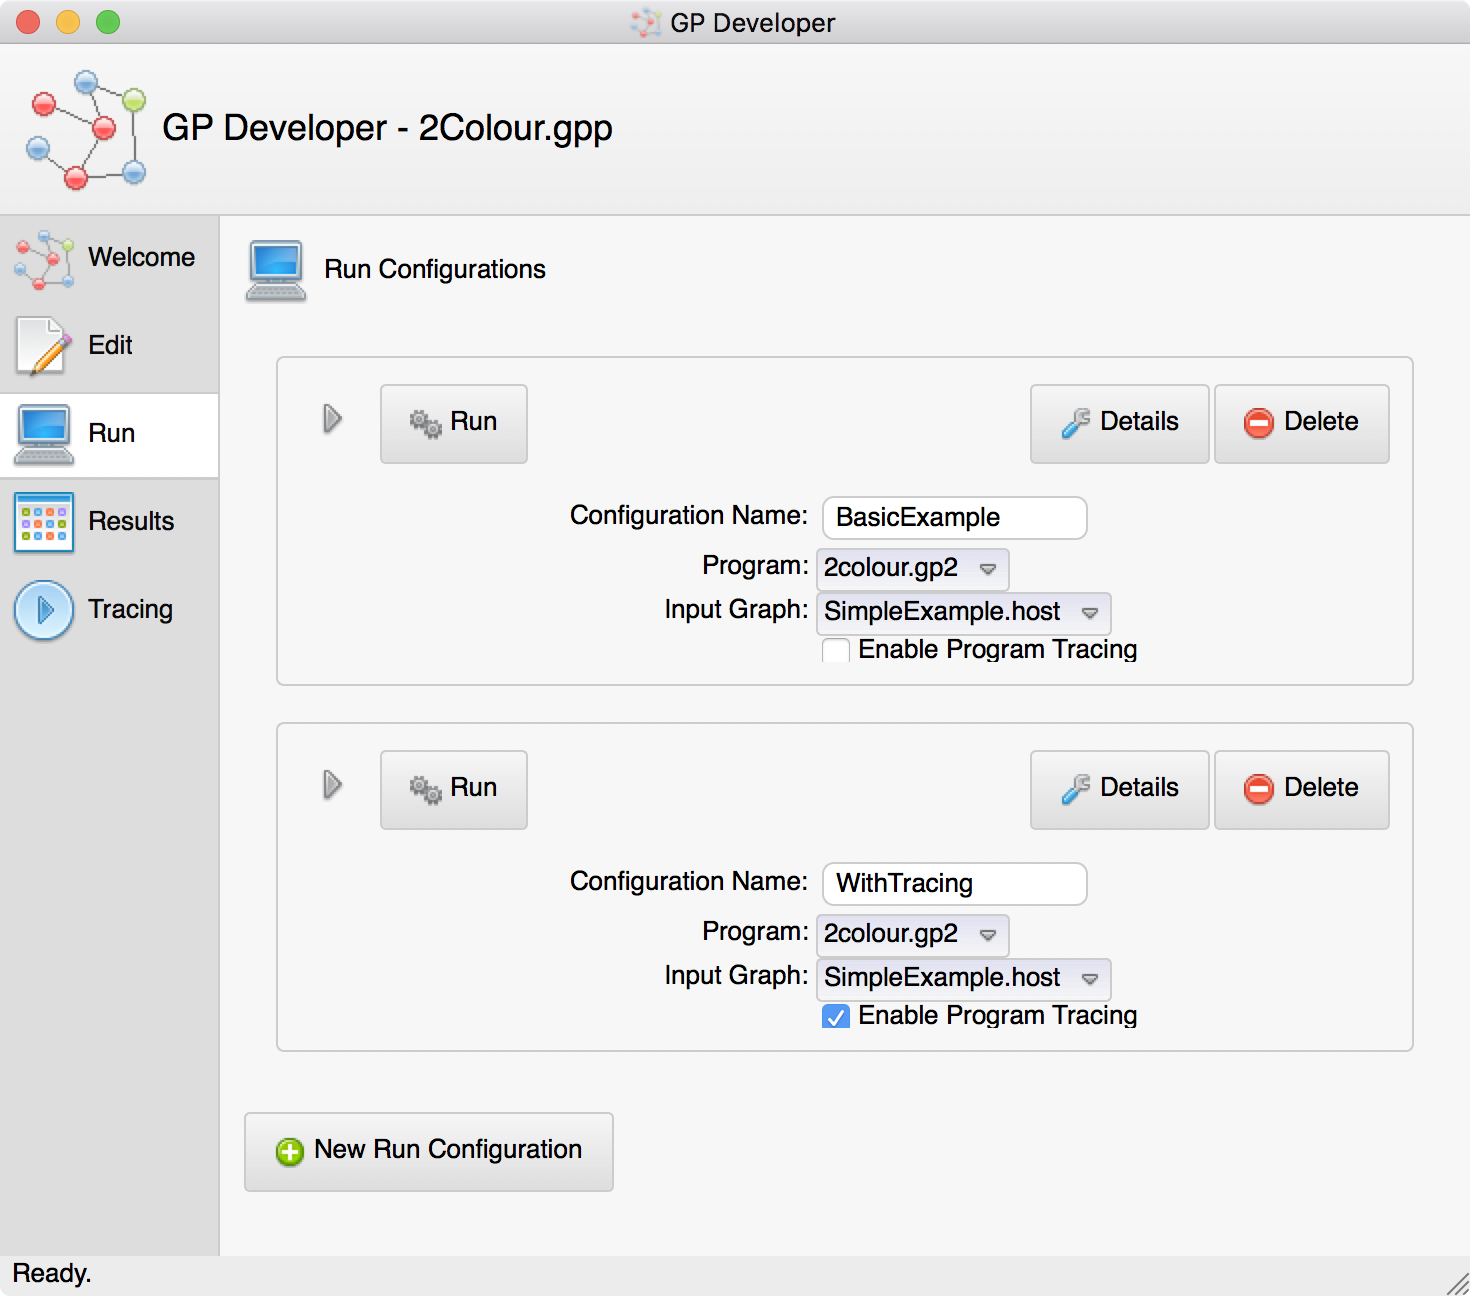
\includegraphics[width=\textwidth]{TracingCheckbox}
    \end{nscenter}
    \caption{Checkbox to enable tracing for a run configuration}
    \label{fig:TracingCheckbox}
\end{figure}

There are two changes in the IDE's UI. First, a checkbox has been added for each
run configuration in the Run tab, shown in \autoref{fig:TracingCheckbox}. Enabling
this checkbox before running a run configuration sets the new compiler command-line
argument to enable tracing for that run. If the checkbox is disabled, the program
runs without tracing, resulting in identical behaviour to before the IDE was
modified. This means the user is free to use the IDE without being forced to run
tracing.

\begin{figure}[!htb]
    \begin{nscenter}
        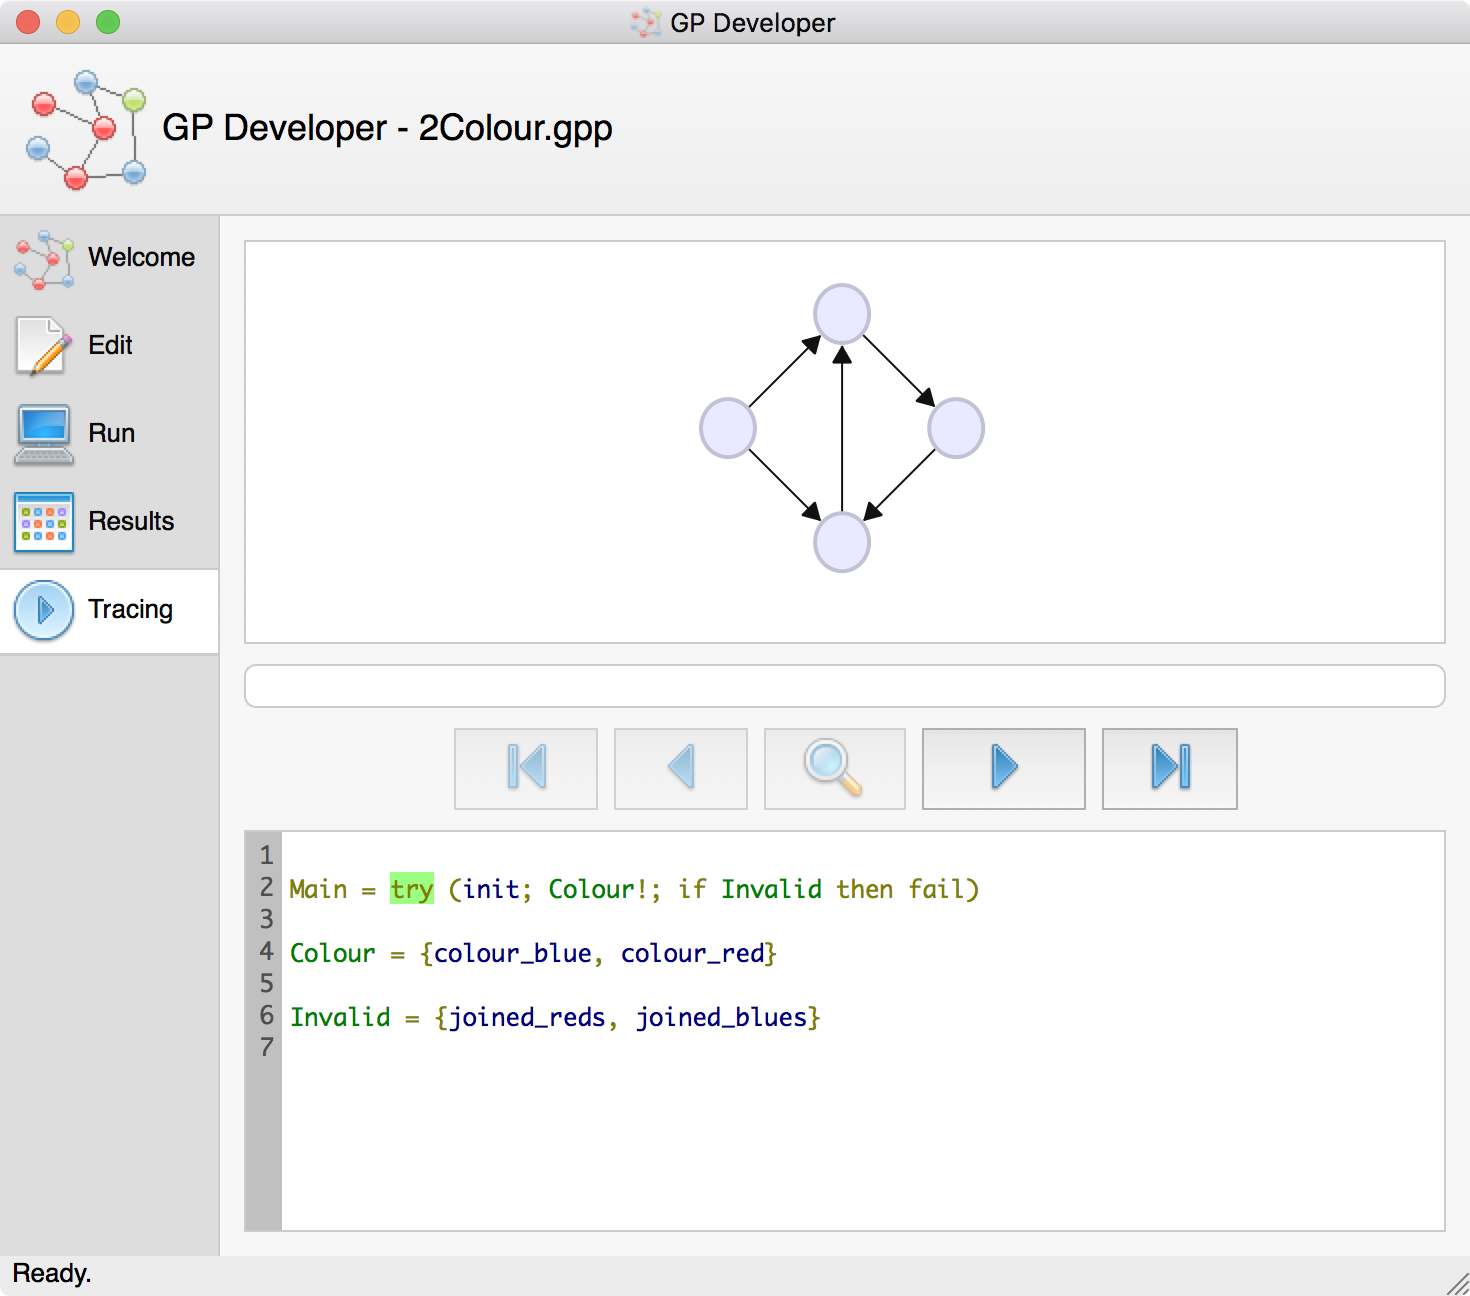
\includegraphics[width=\textwidth]{TracingTab}
    \end{nscenter}
    \caption{Tracing tab in the IDE}
    \label{fig:TracingTab}
\end{figure}

The other modification was to add a new tab to the left side of the window
which, when clicked, opens a screen where the user can view and control the trace.
This screen is shown in \autoref{fig:TracingTab}.

At the top of this screen is the graph at the current point in the trace. This
graph view is updated whenever the user steps forward or backward in the trace,
to reflect the graph as it would have appeared if the program ended at that point.

Below the graph view is a status bar, a small line of text which is updated to
give the user information about the state of the program. For example, when a rule
fails to match, a message is displayed in the status bar. The status bar is necessary
because some situations, such as failed rule matches, cannot be displayed on the graph
or in the program text, since there is no well-defined or clear way to do so.

Next is a row of buttons which are used to control the trace. It is possible to
step forward and backward by one step, or to jump directly to the beginning or the
end of the trace. There is also a button which highlights a rule match, if there
is a valid match. The match is shown in the graph view by highlighting the nodes
and edges which comprise the match. The button then changes to allow the user to
apply the rule on the match being shown.

Finally, at the bottom of the screen, there is a copy of the program text. In this
section, the next step of the program is highlighted with a green background. This
shows the user what will be executed if they press the ''Step Forward'' button. Some
IDEs, such as Visual Studio, display a marker on the left edge of the program text
to show the next line of code which will be executed. This would not work for GP2,
because there may be multiple rule calls on a single line of a GP2 program, and it
is important to distinguish which one is the next to be called. This is why the
individual program tokens must be highlighted, instead of the entire line.

\subsection{Tracing Backend}
\label{sec:TracingBackend}

To support reading tracefiles and displaying the trace in the UI, five new
components were added to the IDE. These components were designed using the
Model-View-Controller (MVC) pattern \citep{mvc}. The \emph{model} reads the
tracefile and tracks the state of the trace, and is formed of three of the
five new components. The other two components are the \emph{view}, which
controls what is shown on-screen, and the \emph{controller}, which handles
communication between the view and the model.

Using MVC makes the system easier to maintain and modify; for example, if a bug
is discovered in the model related to parsing the tracefile, the view component
does not need to be modified, since the view simply updates the user interface
based on the data it receives from the controller.

\subsubsection{Model}
\label{sec:MVCModel}

The model is made up of three C++ classes, each with a specific task. This
modularity means that functionality is encapsulated within an object designed
to perform that specific function, increasing the readability and maintainability
of the system.

\begin{itemize}
    \item The \texttt{TraceParser} class is responsible for reading the tracefile
          and determining the steps the program took while it was running. It is
          implemented using the Qt class \texttt{QXMLStreamReader}, which
          parses an XML document from a data stream; it does not require an entire XML file
          to begin the parsing process. This is useful because it means the
          IDE can handle tracing even from a program which crashed or was forced
          to terminate early, even though the end of the tracefile will be missing
          in these cases.

          Each time the \texttt{TraceParser} is called, it parses one XML tag, such
          as a \texttt{<procedure>} context, or a graph change such as a
          \texttt{<createdNode>} element. This tag is then converted into a custom
          C++ \texttt{TraceStep} structure which contains all the information about
          that step in the trace, including the type of step, any changes made to
          the graph during that step, and the name of the context. These structures
          are then stored in a list, in order, so that iterating over the list steps
          through the trace.

    \item The \texttt{TraceHighlighter} class is used to determine which part of
          the program text should be highlighted in the UI. Its \texttt{update()}
          method takes a \texttt{TraceStep} structure as an argument, which is used
          to find the matching portion of the program text.

          For instance, if it is passed a \texttt{TraceStep} object representing a
          rule call, it starts from the current highlighted position and searches
          through the program looking for a call to a rule with the same name. Since
          GP2 programs are executed in textual order, the first matching rule call it
          finds must be the correct one.

          When a \texttt{TraceStep} is passed in which represents the beginning or
          end of a context (as defined in Section~\ref{sec:TracingModule}), it searches
          for GP2 keywords, such as \texttt{if}, \texttt{try}, or \texttt{skip}, or
          symbols, such as the loop operator \texttt{!} or curly braces \texttt{\{}
          \texttt{\}} for a ruleset.

    \item Finally, the \texttt{TraceRunner} class stores the state of the trace, and
          calls the \texttt{TraceParser} and \texttt{TraceHighlighter} classes when
          required. It is this class which handles method calls from the controller,
          either to step through the trace in a specified direction or to find and
          highlight a match for the current rule.

          When the \texttt{step()} method is called, it attempts to load the next
          \texttt{TraceStep} structure from the list. If there are none left in the
          list, the \texttt{TraceParser} class is called in order to parse the next
          step of the trace. The parsing is done incrementally in this way to increase
          performance and reduce memory usage; parsing the entire tracefile may take
          a significant amount of time if the program had a large number of steps, and
          each of these steps would need to be stored in the list. By parsing
          incrementally, trace steps are only parsed and stored when the user reaches
          them in the trace, so if they exit the trace before the end, the parser did
          not waste time parsing the end of the XML.

          After loading the next \texttt{TraceStep}, any graph changes from that step
          are applied to the graph. If the user is stepping backwards through the trace,
          the graph changes from the step are reversed; for example, if a node was
          added at that point, stepping backwards would remove the node from the graph.
          The \texttt{TraceRunner} class exposes a \texttt{getGraph()} method to return
          the current graph state for displaying in the UI; the controller calls this
          method when the user clicks a button to step through.

          Finally, the \texttt{TraceStep} \emph{after} the current one is then passed
          to the \texttt{TraceHighlighter}, which returns the position in the program
          which should be highlighted. As previously discussed, the next step is
          highlighted, not the step which was just executed, so that the user is aware
          of what will occur when they click the step button.

\end{itemize}

\subsubsection{View}
\label{sec:MVCView}

The view is a Qt \emph{form}, a special file format which tells the Qt
framework which UI elements to display and how to display them. The view
component does not contain any code; it simply describes how to build the UI as
outlined in Subsection~\ref{sec:UIChanges}.

\subsubsection{Controller}
\label{sec:MVCController}

The controller is a small C++ class which acts as a communication layer between
the view and the model. When the user clicks a button in the view, the controller
forwards a method call onto the model, performing the action intended by the
button which was pressed.

At the end of the method call linked to each button, the controller fetches the
most recent graph and program highlight state from the \texttt{TraceRunner}, and
uses it to update the view.

\clearpage

%XXXXXXXXXXXXXXXXXXXXXXXXXXXXXXXXXXXXXXXXXXXXXXXXXXXXXXXXXXXXXXXXXXXXXXXXXXXXXX

\chapter{Evaluation}
\label{cha:Evaluation}

\section{Requirements Tracing}
\label{sec:RequirementsTracing}

To evaluate the new functionality added to GP2, the implementation has been
compared to the list of requirements outlined in Section~\ref{sec:ListOfRequirements}.
\autoref{tab:RequirementsTracing} lists each of the requirements, along with whether
that requirement has been met by the system.

\begin{table}[!htb]
    \begin{tabularx}{\linewidth}{|l|l|X|}
        \hline
        \textbf{ID} & \textbf{State} & \textbf{Summary} \\ \hline
        1    &  Implemented     & A GP2 program can be traced from start to end, producing
                                  the same result as the original output. \\ \hline
        1.1  &  Implemented     & The ''Step Forward'' button applies one rule at a time. \\ \hline
        1.2  &  Implemented     & The trace can be reversed to step backwards through the
                                  program. \\ \hline
        1.3  &  Not Implemented & It is only possible to step rule-by-rule, or to jump to
                                  the beginning or end of the trace. There is no way to
                                  execute an entire loop, for instance. \\ \hline

        2    &  Implemented     & The GP2 IDE contains a Tracing tab which is used to
                                  visually trace a program's execution. \\ \hline
        2.1  &  Implemented     & Rule calls are highlighted in the program text when they
                                  are executed in the trace. \\ \hline
        2.2  &  Implemented     & The ''Find Match'' button highlights the match for the
                                  current rule. However, this is a manual operation; the
                                  match is not highlighted for every step unless requested
                                  by the user. \\ \hline
        2.3  &  Implemented     & The program text is highlighted in the Tracing tab to
                                  show the current position. \\ \hline
        2.4  &  Not Implemented & The system has no way to highlight which changes were made
                                  by the previous rule application. \\ \hline
        2.5  &  Implemented     & Whenever the graph changes, the latest graph is shown in
                                  the IDE. \\ \hline

        3    &  Implemented     & The user can control tracing using buttons in the tracing
                                  tab of the IDE. \\ \hline
        3.1  &  Implemented     & The ''Step Forward'' button advances the trace by one
                                  step. \\ \hline
        3.2  &  Implemented     & The ''Step Backward'' button reverses the trace by one
                                  step. \\ \hline
        3.3  &  Implemented     & The ''Find Match'' button highlights the match for the
                                  next rule. \\ \hline
        3.4  &  Implemented     & When the ''Find Match'' button is used, it becomes an
                                  ''Apply Match'' button, which completes the application
                                  of the rule. \\ \hline
        3.5  &  Implemented     & Tracing can be disabled using the checkbox in the Run tab.
                                  \\ \hline
                
        4    &  Implemented     & GP2 programs behave identically when tracing is enabled
                                  and disabled, since all code changes are additive and did
                                  not modify existing behaviour. \\ \hline
        4.1  &  Implemented     & Enabling tracing simply outputs a tracefile during execution,
                                  and does not change the behaviour of the program. The results
                                  are identical whether tracing is enabled or disabled. \\ \hline
        4.2  &  Implemented     & When old projects are loaded, tracing is disabled by
                                  default for each run configuration. Nothing else needs
                                  to be modified to run old programs. \\ \hline
                
    \end{tabularx}
    \caption{State of each of the previously defined system requirements}
    \label{tab:RequirementsTracing}
\end{table}

All of the must-have system requirements have been implemented, meaning that the
system successfully implements a debugging tool for GP2 programs. The two
unimplemented requirements were defined as ''desirable'' and were not essential
for the tool to be useable.

%//////////////////////////////////////////////////////////////////////////////

\section{Maintainability}
\label{sec:MaintainabilityEval}

Some key goals were set out in Section~\ref{sec:IntegrationAndMaintainability}
related to the maintainability of the system. Throughout the project, any
modifications being made to the system were designed with ease of understanding
in mind. The newly added code follows the conventions set out by the existing
GP2 code, and all new code has comments. Semantic names were chosen for variables,
functions, and methods to ensure future developers who are unfamiliar with the
changes can understand what the code does.

Careful thought was applied to ensure that tracing was optional when compiling
and running a GP2 program, and that the new code did not create strong 
dependencies between components. This has been achieved by separating the
tracing components into separate modules, both in the compiler and the IDE,
meaning they could easily be removed or changed without affecing the behaviour of
the rest of the system.

%//////////////////////////////////////////////////////////////////////////////

\section{Performance}
\label{sec:Performance}

\begin{table}[!htb]
    \begin{nscenter}
        \begin{tabular}{|l|r|r|}
            \hline
            \textbf{Tracing} & \textbf{Average Compilation Time (ms)} & \textbf{Average Run Time (s)} \\ \hline
            Disabled         & 9.6                                    & 12.970                        \\ \hline
            Enabled          & 10.0                                   & 15.180                        \\ \hline
        \end{tabular}
        \caption{Average performance of the 11th-generation Sierpinski Triangle program}
        \label{tab:PerformanceTests}
    \end{nscenter}
\end{table}

It is important that the changes made to GP2 did not negatively impact the speed
of compiling and running a program, since it would make debugging a program
cumbersome to have to wait longer for the program to execute.

To check the performance of the system, the Sierpinski Triangle generation
program mentioned in Section~\ref{sec:ChosenSolution} was compiled and run with
tracing disabled and then with tracing enabled, to compare the time taken in
both cases. The program was set to generate the 11th-generation Sierpinski
Triangle.

In each case, the program was compiled and run ten times, and the average time
was taken. These tests were run on a PC with a 4.0 GHz processor and 24 GB of RAM
using the UNIX \texttt{time} facility to measure the time taken.

The results of these tests are shown in \autoref{tab:PerformanceTests}. There
is very little difference between the compilation times, as expected, since compiling
a program with tracing simply adds some additional function calls to the compiled
C program.

At runtime, the program with tracing enabled runs for approximately 17\% longer
than the program with tracing disabled. This is due to the program writing trace
data to the filesystem at each step. A performance decrease of 17\% is fairly small,
and would probably not be noticeable for small programs with short runtimes. For
larger programs which may take a minute or longer to run, the performance impact
may be concerning, since it would be much more noticeable.

It may be desirable for future work to be done on the tracing component in order
to reduce the performance impact. However, as an initial implementation, a 17\%
impact is acceptable, and the system is still reasonable to use, especially for
small GP2 programs.

\clearpage

%XXXXXXXXXXXXXXXXXXXXXXXXXXXXXXXXXXXXXXXXXXXXXXXXXXXXXXXXXXXXXXXXXXXXXXXXXXXXXX

\chapter{Conclusions}
\label{cha:Conclusions}

In this project, a need was identified for a way to closely follow the execution
of a GP2 program, in order to find bugs or improve understanding. To fulfil this
requirement, the ability to trace a GP2 program was added to the compiler, and
a way to read and follow traces was added to the IDE.

When tracing is enabled in the compiler, additional function calls are added to
the compiled program, each of which prints some data about the running program
to an XML tracefile. Enough of these function calls are made throughout the
execution of the program so that the tracefile contains enough information to
fully recreate the actions taken by the program, after the program has finished
running.

In the IDE, a new module was added which parses the tracefile created by the
program, and uses this to display the intermediate states of the program to the
user. The user is able to step through the trace, both forwards and backwards,
and see how the graph changes as the program progresses. The tracing section of
the IDE also highlights the current position in the program text, and has the
ability to highlight the nodes and edges in the graph which make up the match
for a given rule call.

The newly implemented system meets all the must-have requirements to be able to
fully trace a program's execution. It also meets some additional non-essential
requirements, such as being able to step backwards, to allow the user to see
part of the program again without having to restart from the beginning.

Overall, this project has been a success, and has achieved the goals which were
set out. The tracing system is entirely functional and brings substantial
improvements to the way GP2 programs can be reasoned about and debugged.


%//////////////////////////////////////////////////////////////////////////////

\section{Future Work}
\label{sec:FutureWork}

\emph{What's missing (e.g. what requirements weren't met) and what other
improvements could be made by someone else?}

\clearpage

%XXXXXXXXXXXXXXXXXXXXXXXXXXXXXXXXXXXXXXXXXXXXXXXXXXXXXXXXXXXXXXXXXXXXXXXXXXXXXX

\bibliography{references}

\end{document}
